%%% ======= Beamer ======
\documentclass[usenames,dvipsnames,t]{beamer}
% \documentclass[usenames,dvipsnames, handout]{beamer}
\beamertemplatenavigationsymbolsempty % remove toolbar at the bottom of slides
\usepackage{appendixnumberbeamer} % for appendix
\usetheme{Madrid}
\usecolortheme{default}
\useinnertheme{circles}

\usepackage{fontawesome}

% Define commands for social media icons with links
\newcommand{\twitter}{\href{https://twitter.com/ThibeauWouters}{\textcolor{black}{\faTwitter}}}
\newcommand{\linkedin}{\href{https://www.linkedin.com/in/ThibeauWouters}{\textcolor{black}{\faLinkedin}}}
\newcommand{\github}{\href{https://github.com/ThibeauWouters}{\textcolor{black}{\faGithub}}}
\newcommand{\myemail}{\href{mailto:t.r.i.wouters@uu.nl}{\textcolor{black}{\faEnvelope}}}
\definecolor{customblue}{HTML}{7db8dc}

\setbeamercolor{author in head/foot}{bg=blue!10, fg=blue}
\setbeamercolor{title in head/foot}{bg=blue!10, fg=blue}
\setbeamercolor{date in head/foot}{bg=blue!10, fg=blue}

\makeatletter
\setbeamertemplate{footline}{
  \leavevmode%
  \hbox{%
  \begin{beamercolorbox}[wd=.333333\paperwidth,ht=2.25ex,dp=1ex,center]{author in head/foot}%
    \usebeamerfont{author in head/foot}\insertshortauthor\expandafter\ifblank\expandafter{\beamer@shortinstitute}{}{~~(\insertshortinstitute)}
  \end{beamercolorbox}%
  \begin{beamercolorbox}[wd=.333333\paperwidth,ht=2.25ex,dp=1ex,center]{title in head/foot}%
    \usebeamerfont{title in head/foot}\insertshorttitle
  \end{beamercolorbox}%
  \begin{beamercolorbox}[wd=.333333\paperwidth,ht=2.25ex,dp=1ex,right]{date in head/foot}%
    \usebeamerfont{date in head/foot}\insertshortdate{}\hspace*{2em}
    \insertframenumber{}%
%     / \inserttotalframenumber
    \hspace*{2ex} 
  \end{beamercolorbox}}%
  \vskip0pt%
}
\makeatother

\colorlet{beamer@blendedblue}{blue!70} % change color theme

\usepackage[style=numeric-comp,sorting=none,backend=biber]{biblatex}%<- specify style
\addbibresource{references.bib}%<- specify bib file

\usepackage{svg}


% For appendix
\newcommand{\backupbegin}{
   \newcounter{framenumberappendix}
   \setcounter{framenumberappendix}{\value{framenumber}}
}
\newcommand{\backupend}{
   \addtocounter{framenumberappendix}{-\value{framenumber}}
   \addtocounter{framenumber}{\value{framenumberappendix}} 
}

\setbeamertemplate{bibliography item}{\insertbiblabel} % improved references


% Other preamble stuff:
\usepackage{preamble}

%%% Uncomment for another color palette
% \definecolor{Logo1}{rgb}{0.0, 0, 0.7}
% \definecolor{Logo2}{rgb}{2.55, 2.55, 2.55}

% \setbeamercolor*{palette primary}{bg=Logo1, fg=white}
% \setbeamercolor*{palette secondary}{bg=Logo2, fg=white}
% \setbeamercolor*{palette tertiary}{bg=white, fg=Logo1}
% \setbeamercolor*{palette quaternary}{bg=white,fg=white}
% \setbeamercolor{structure}{fg=Logo1} % itemize, enumerate, etc
% \setbeamercolor{section in toc}{fg=Logo1} % TOC sections

% For figures
\usepackage{import}
\usepackage{xifthen}
\usepackage{pdfpages}
\usepackage{transparent}
\usepackage{mdframed}
\usepackage{subcaption}

\setbeamertemplate{caption}[numbered]


% --- Inkscape figures:
\newcommand{\incfig}[2][0.75\textwidth]{%
    \def\svgwidth{\columnwidth}
    \resizebox{#1}{!}{\import{Inkscape/}{#2.pdf_tex}}
}

% --- Height of frame
\newlength{\myheight}
\setlength{\myheight}{7cm}

\newlength\myheightfigureintext
\newlength\mydepthfigureintext
\settototalheight\myheightfigureintext{Xygp}
\settodepth\mydepthfigureintext{Xygp}
\setlength\fboxsep{0pt}


%------------------------------------------------------------
%This block of code defines the information to appear in the
%Title page
\title[BNS in ET] %optional
{Scalable and sequential inference of the neutron star equation of state with the Einstein Telescope}

\author[Thibeau Wouters]{Thibeau Wouters \\ \vspace{2mm} \href{mailto:t.r.i.wouters@uu.nl}{t.r.i.wouters@uu.nl} \newline \github \quad \linkedin \quad \myemail}

% \raisebox{-\mydepthfigureintext}{\fbox{\includegraphics[height=\myheightfigureintext]{Figures/arxiv_logo_red_no_background.png}}}

\date{BeNL meeting 2026}



%End of title page configuration block
%------------------------------------------------------------



%------------------------------------------------------------
%The next block of commands puts the table of contents at the 
%beginning of each section and highlights the current section:

% \AtBeginSection[]
% {
%   \begin{frame}[plain, noframenumbering]
%     \frametitle{Table of Contents}
%     \tableofcontents[currentsection]
%   \end{frame}
% }


%------------------------------------------------------------


\begin{document}

{

\usebackgroundtemplate{\transparent{0.5}{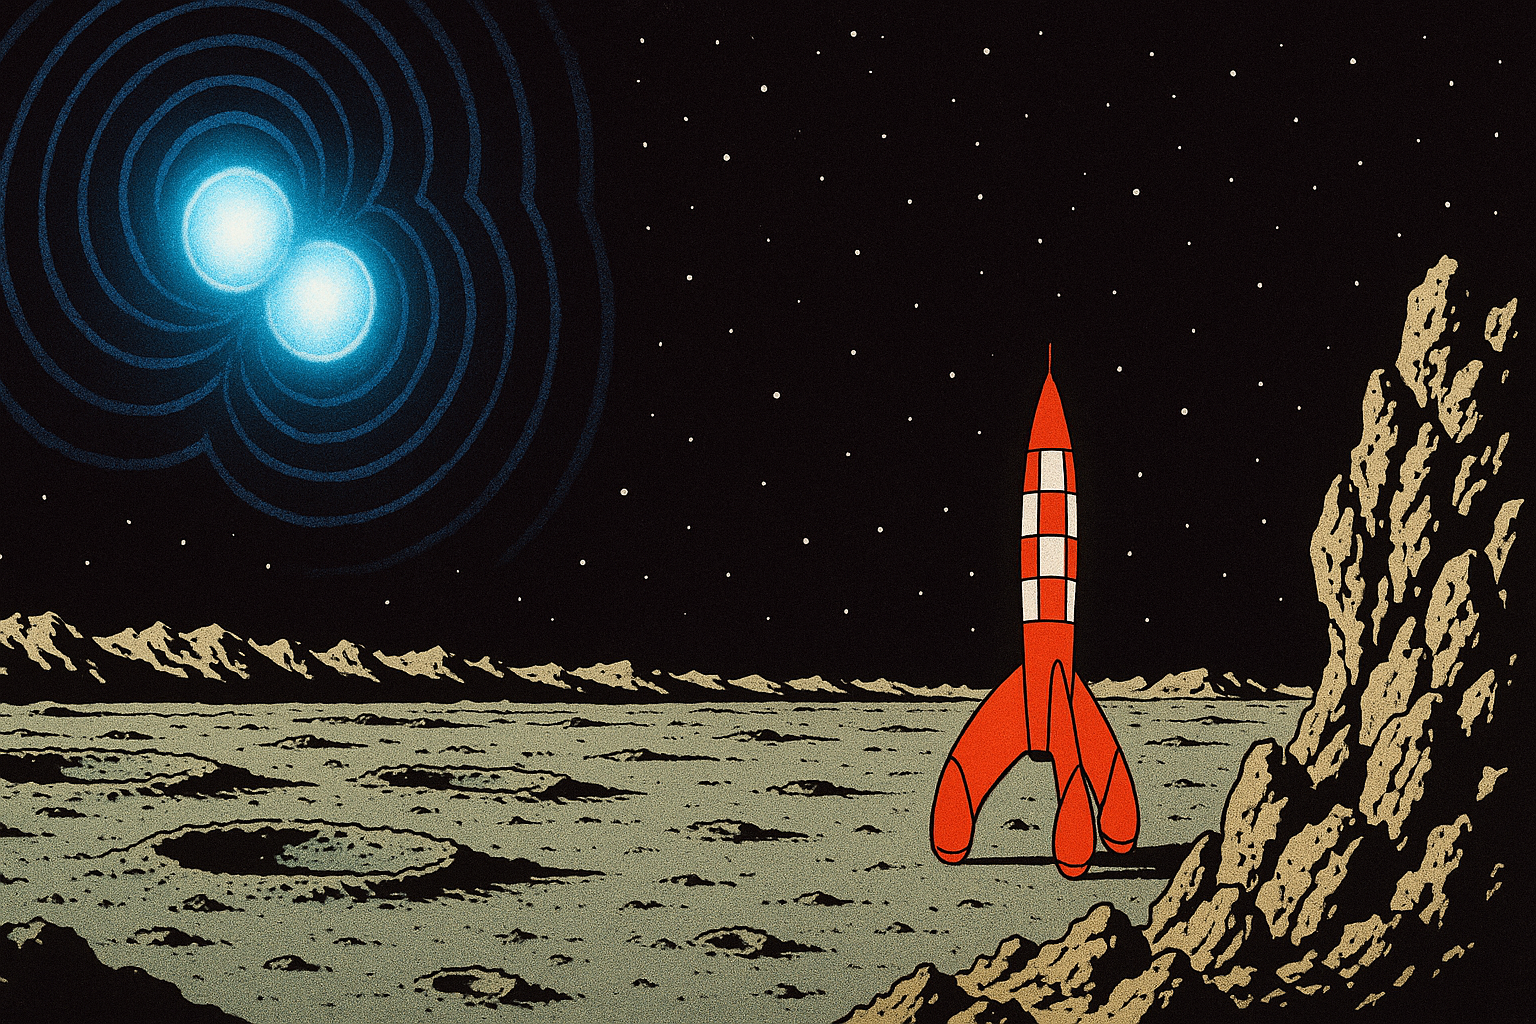
\includegraphics[width=\paperwidth,height=\paperheight]{Figures/tintin_BNS_2.png}}}

\begin{frame}[plain, noframenumbering]

  \begin{tikzpicture}[remember picture,overlay]
    \node[fill=customblue, fill opacity=0.75, text opacity=1, rounded corners=10pt, inner sep=15pt] at (current page.center) {
      \begin{minipage}{0.85\textwidth}
        \centering
        \normalsize\mdseries Scalable and sequential inference of the neutron star equation of state with the Einstein Telescope \\[1.5ex]
        Thibeau Wouters \\[0.5ex]
        \normalsize \github \quad \linkedin \quad \myemail
      \end{minipage}
    };
  \end{tikzpicture}

  \vspace{7cm}

  \begin{columns}
  \column{0.35\textwidth}
  \begin{figure}
    \centering
    \vspace{1.5mm}
    
\includegraphics[width=0.75\linewidth]{Figures/utrecht-university.png}
  \end{figure}
  \column{0.35\textwidth}
  \begin{figure}
    \centering
    
\includegraphics[width=0.75\linewidth]{Figures/Nikhef_logo-transparent.png}
  \end{figure}
\end{columns}

\end{frame}
}

% %The next statement creates the title page.
% \frame[plain]{\titlepage



% }


%---------------------------------------------------------
%This block of code is for the table of contents after
%the title page
% \begin{frame}[plain, noframenumbering]
% \frametitle{Table of Contents}
% \tableofcontents
% \end{frame}
%---------------------------------------------------------


% \section{Introduction}

\begin{frame}{Neutron stars and fundamental physics}

  Neutron star mergers and multimessenger observations probe
  \vspace{3mm}
  \begin{itemize}
    \item Equation of state of ultradense matter~\cite{LIGOScientific:2018cki}

    \vspace{2mm}

    \item Expansion of the universe ($H_0$)~\cite{LIGOScientific:2017adf}

    \vspace{2mm}
    
    \item Tests of GR, populations, nucleosynthesis,...
  \end{itemize}

  \vspace{3mm}

  \begin{figure}
    \centering
    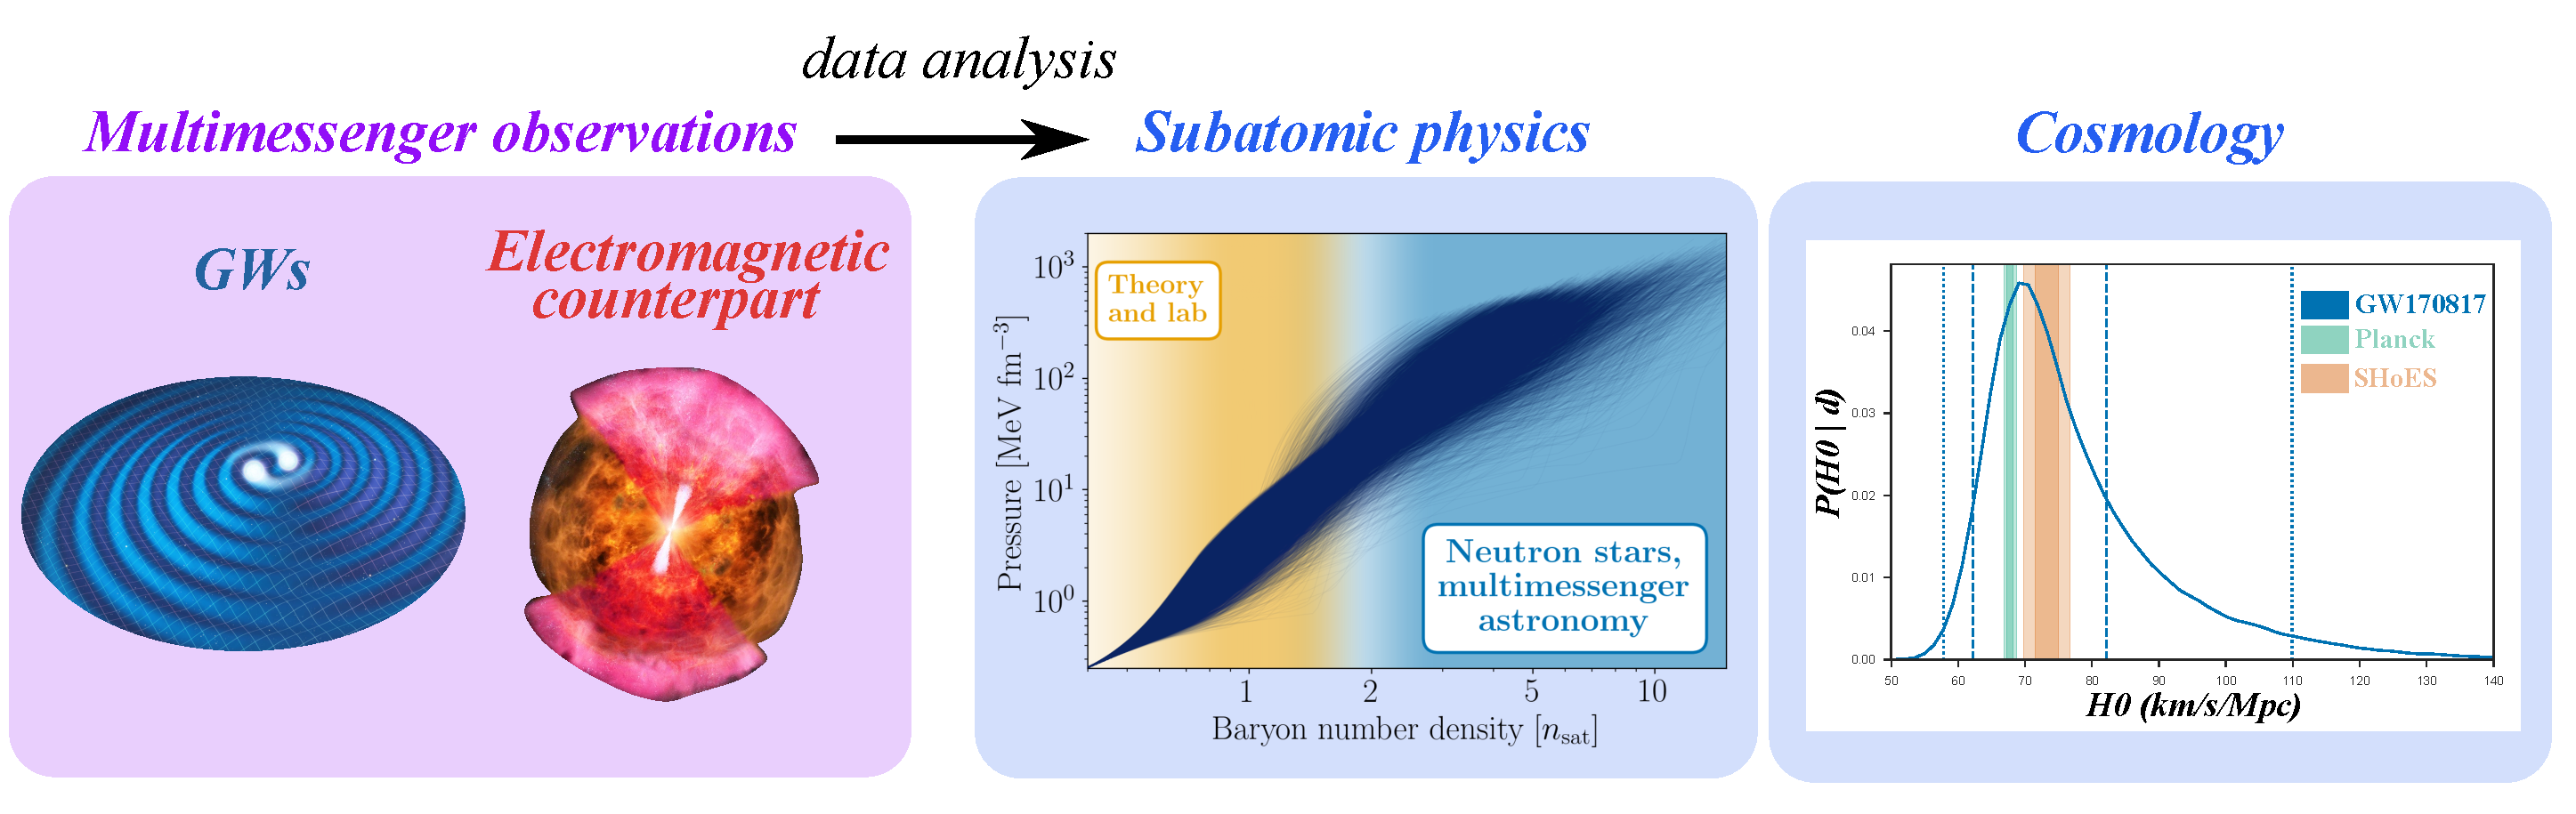
\includegraphics[width=0.99\textwidth]{Inkscape/introduction.pdf}
  \end{figure}
  
\end{frame}

\begin{frame}{Challenges for Einstein Telescope}

  \def\x{3mm}

  \begin{itemize}
    \item Einstein Telescope
    \begin{itemize}
      \item $\sim 30,000$ binary neutron star mergers/year
      \item $\sim 100$ with detected electromagnetic counterpart
    \end{itemize}

    \vspace{\x}

    \item \textbf{Challenge}: Data analysis (Bayesian inference) needs to scale up:
    \begin{itemize}
      \item \jaxdarkgreen{Single-event}: analyze each event independently
      \item \jaxpurple{Population}: combine events into science insights
    \end{itemize}

    \vspace{\x}

    \item \textbf{Solution}: GPU-acceleration $\times$ algorithm innovations
  \end{itemize}

  \begin{figure}
    \centering
    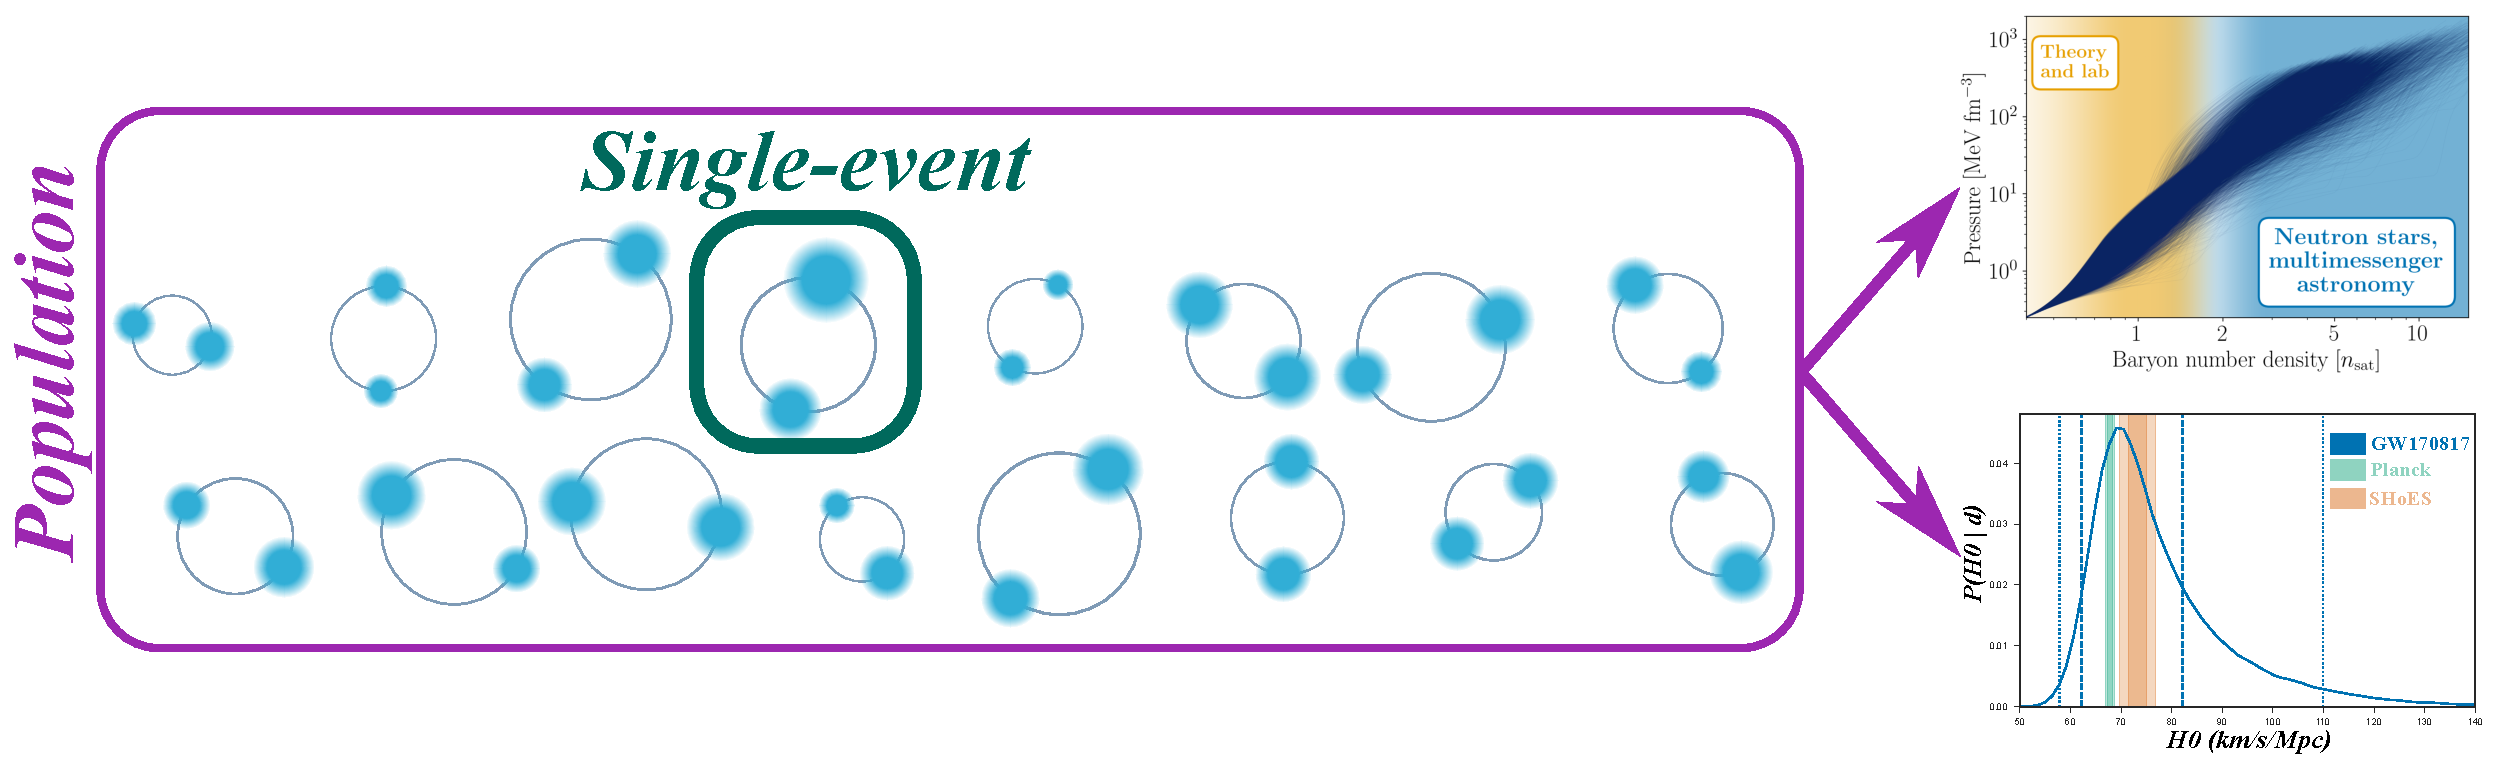
\includegraphics[width=0.9\textwidth]{Inkscape/bns_et.pdf}
  \end{figure}
\end{frame}

\begin{frame}[plain, noframenumbering]{}
  \vspace{20mm}
  \begin{figure}
    \centering
    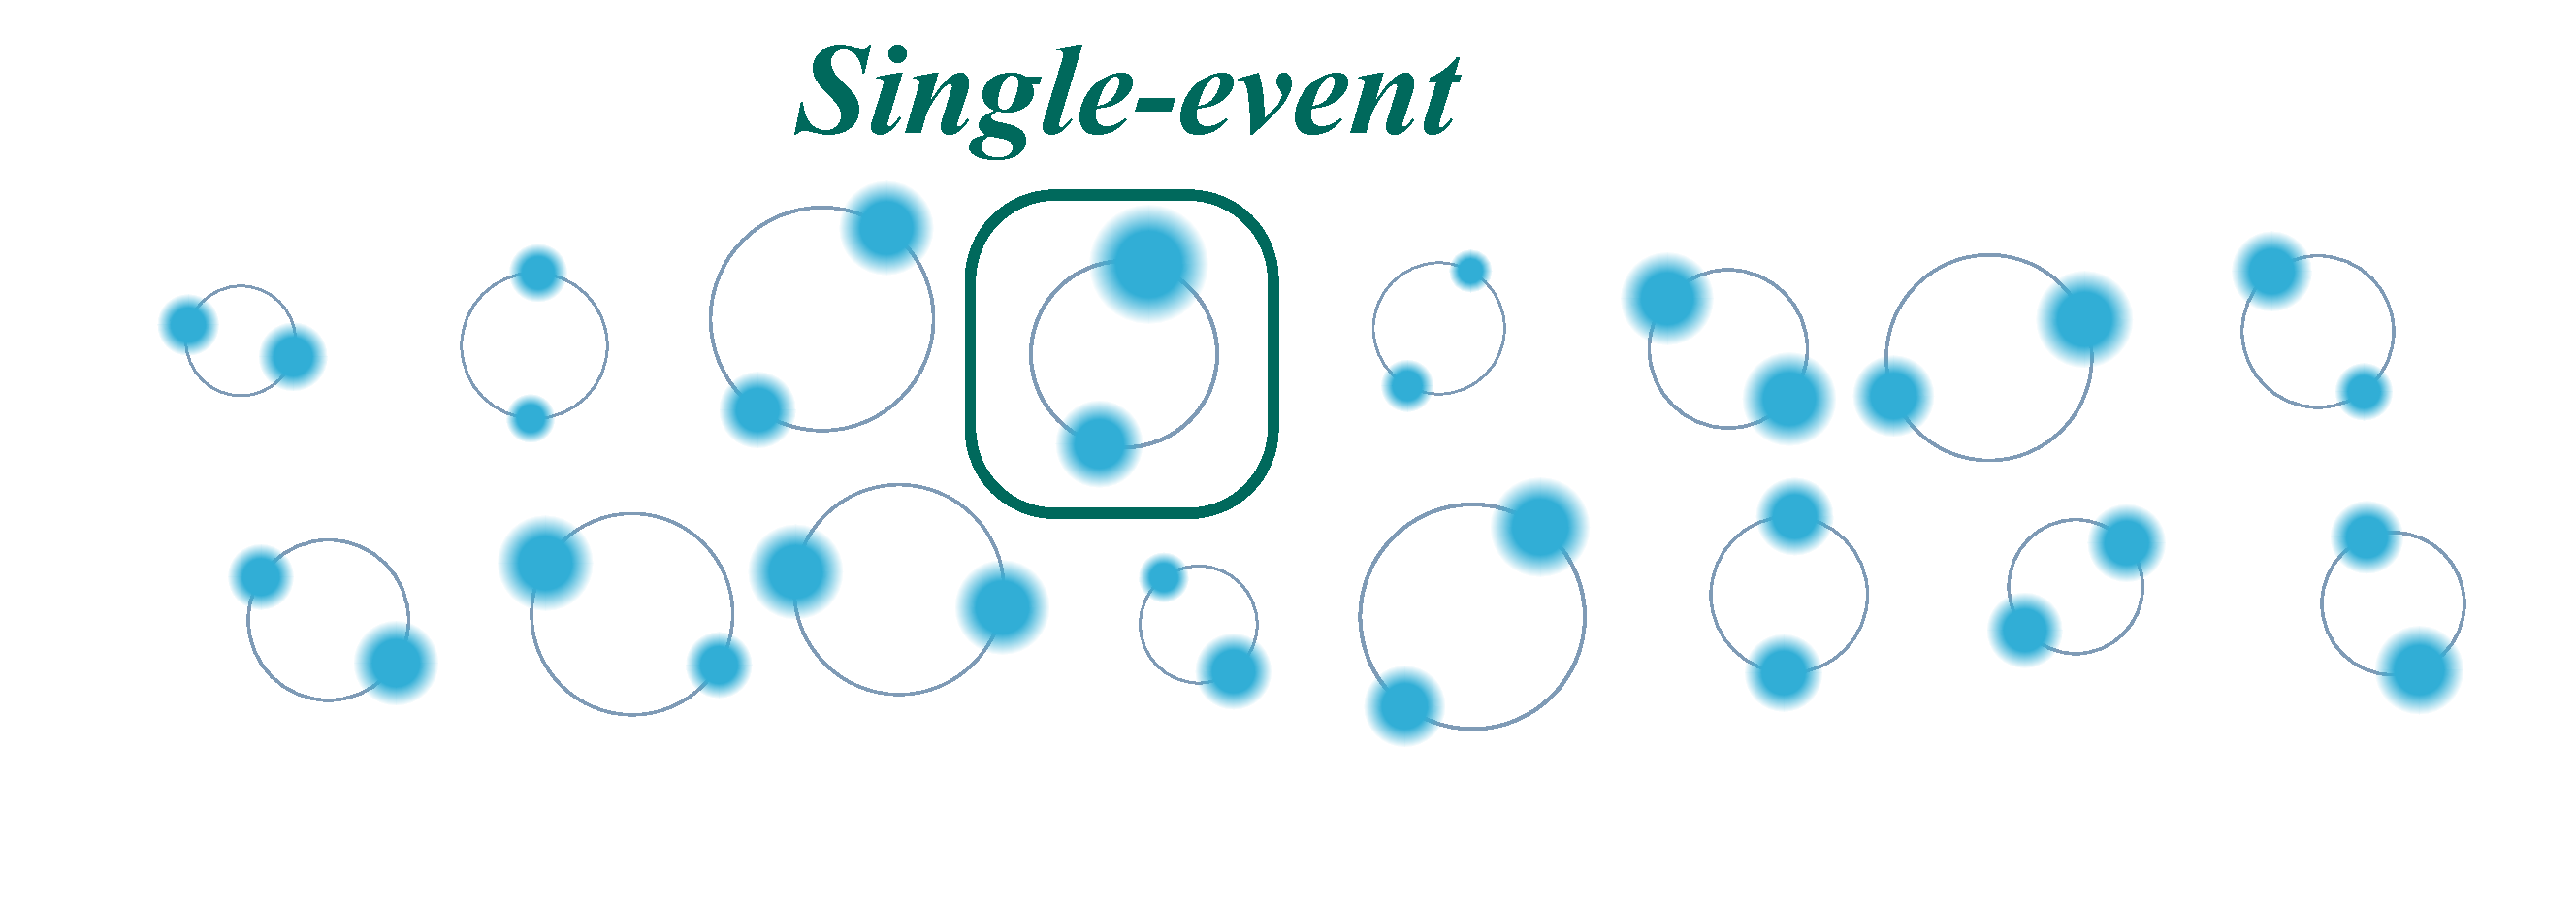
\includegraphics[width=0.9\textwidth]{Inkscape/single_event.pdf}
  \end{figure}
\end{frame}

\begin{frame}{Single event: slice-within-Gibbs sampler (\texttt{2607.28265})}

  \def\x{3mm}
  \def\y{1mm}

  \begin{itemize}
    \item Waveform generation is expensive

    \vspace{\x}

    \item \textbf{Slice-within-Gibbs}~\cite{Yallup:2026nqc}: move in `blocks'
    \begin{itemize}
      \vspace{\y}
      \item \swigyellow{\textbf{Slow}}: new waveform generations, cached

      \vspace{\y}

      \item \swiggreen{\textbf{Fast}}: projections, reuse cache
    \end{itemize}

    \vspace{\x}

    \item Inference (for LVK signals!) in $15$ mins with \textbf{no} approximation, or faster than signal duration ($128$ s) with relative binning
  \end{itemize}

  \begin{figure}
    \centering
    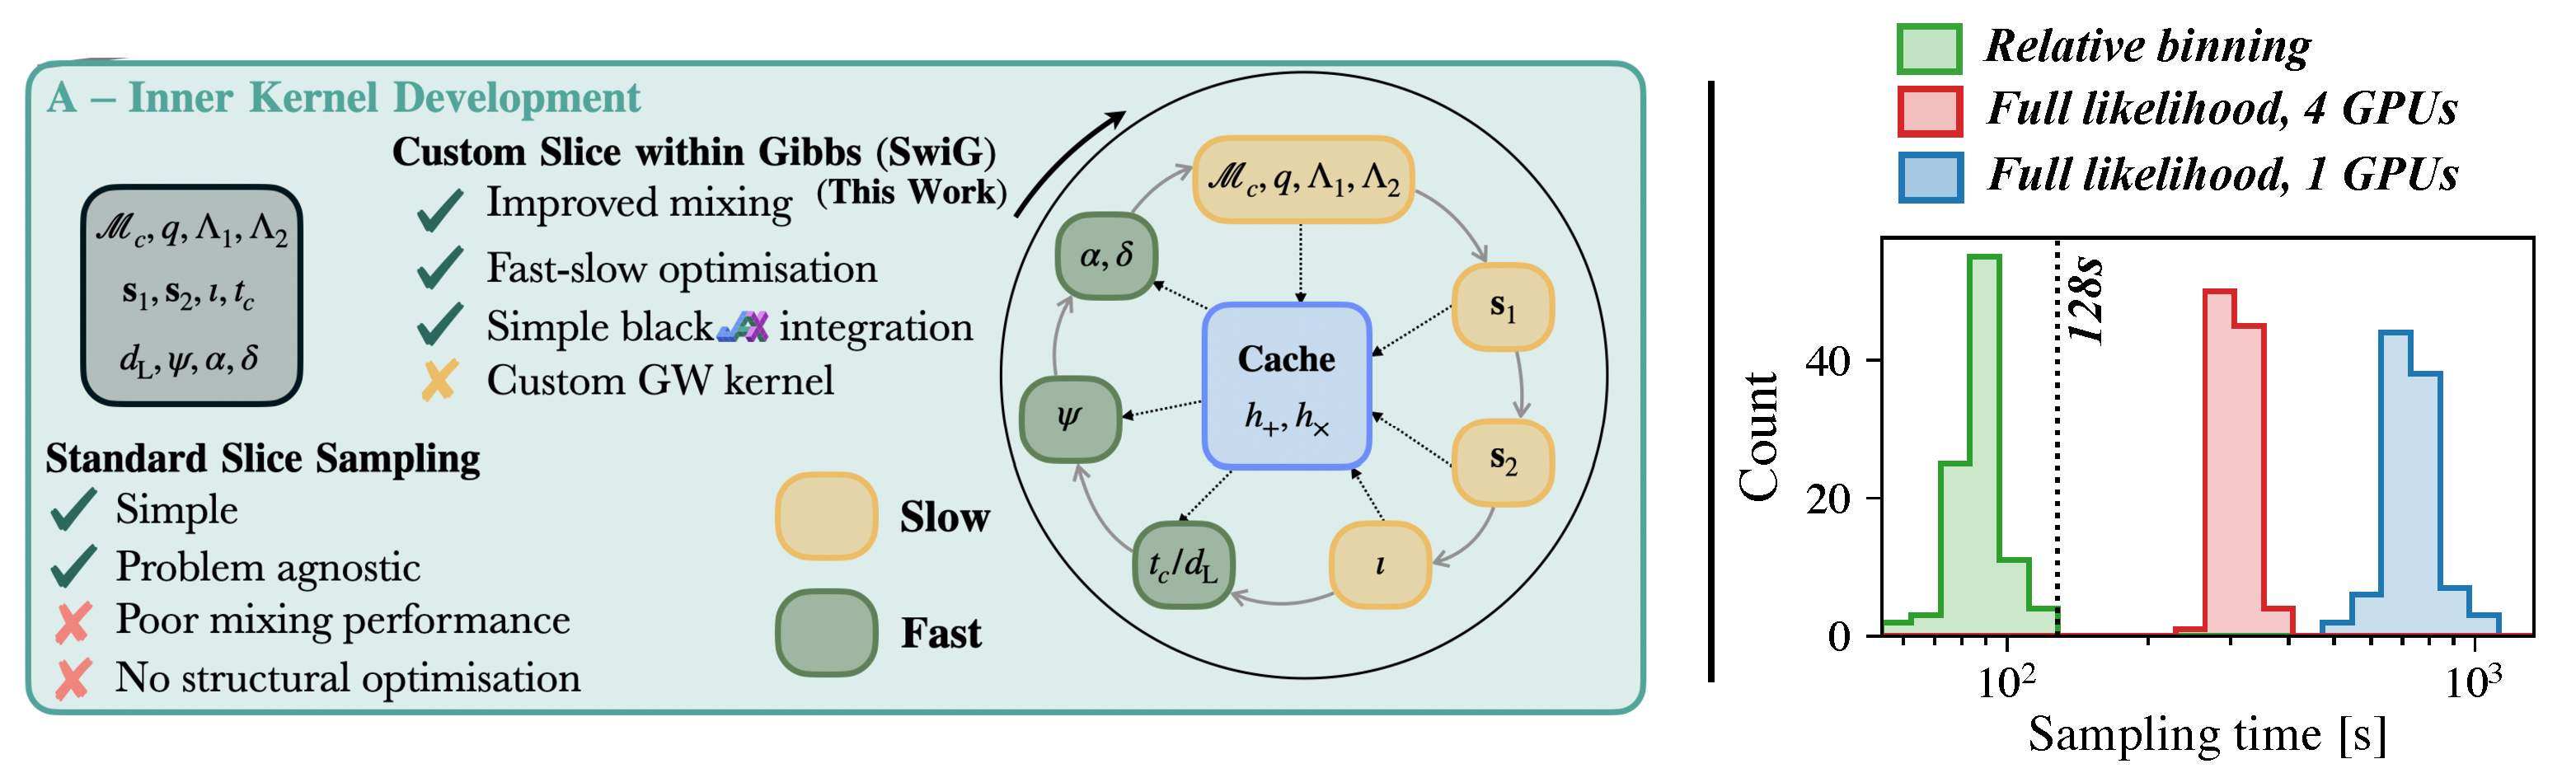
\includegraphics[width=0.975\textwidth]{Inkscape/swig.pdf}
  \end{figure}
\end{frame}

\begin{frame}{Towards ET with the BeNL community}

  \def\x{3mm}
  \def\y{1mm}

  \begin{itemize}
    \item Development extended towards ET signals

    \begin{itemize}
      \vspace{\y}
      \item \textsc{ripple} \href{https://github.com/GW-JAX-Team/ripple}{\textcolor{black}{\faGithub}}: state-of-the-art waveforms (\robintalk{\textbf{talk by Robin}})

      \vspace{\y}
      \item \textsc{jim} \href{https://github.com/GW-JAX-Team/jim}{\textcolor{black}{\faGithub}}: developing samplers (Thomas~C.~K.~Ng)
    \end{itemize}

    \vspace{\x}

    \item Strong BeNL presence (Harsh Narola, Peter T. H. Pang, Fabian Gittins, Isaac~C.~F.~Wong,\dots)
  \end{itemize}

  \begin{figure}
    \centering
    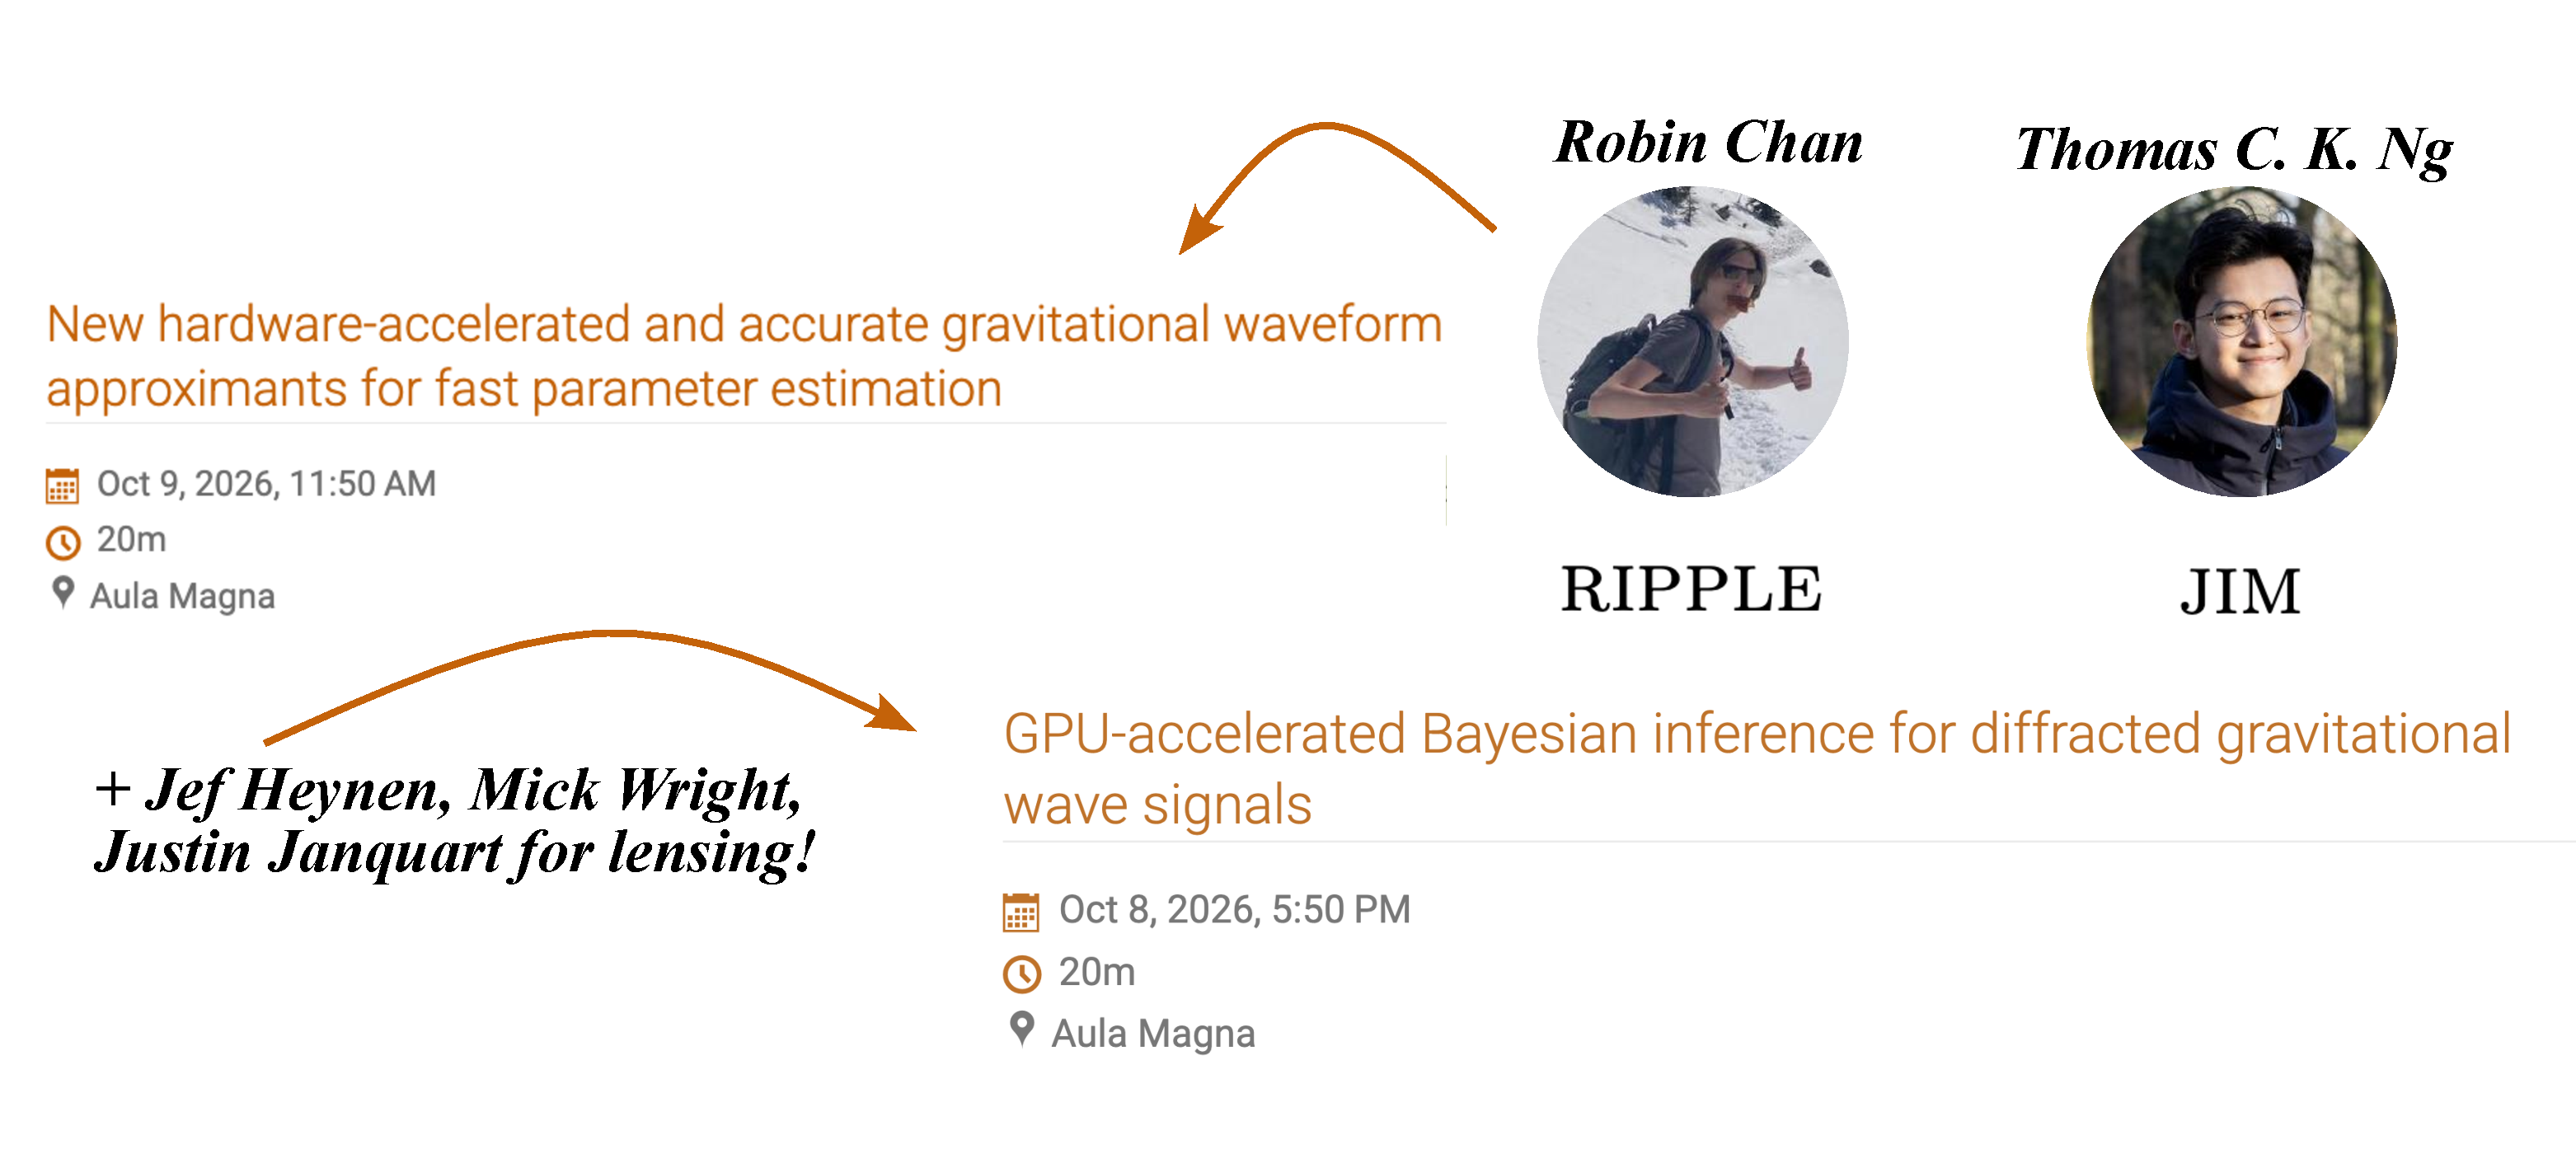
\includegraphics[width=0.975\textwidth]{Inkscape/ripple_and_jim.pdf}
  \end{figure}
\end{frame}

\begin{frame}[plain, noframenumbering]{}
  \vspace{10mm}
  \begin{figure}
    \centering
    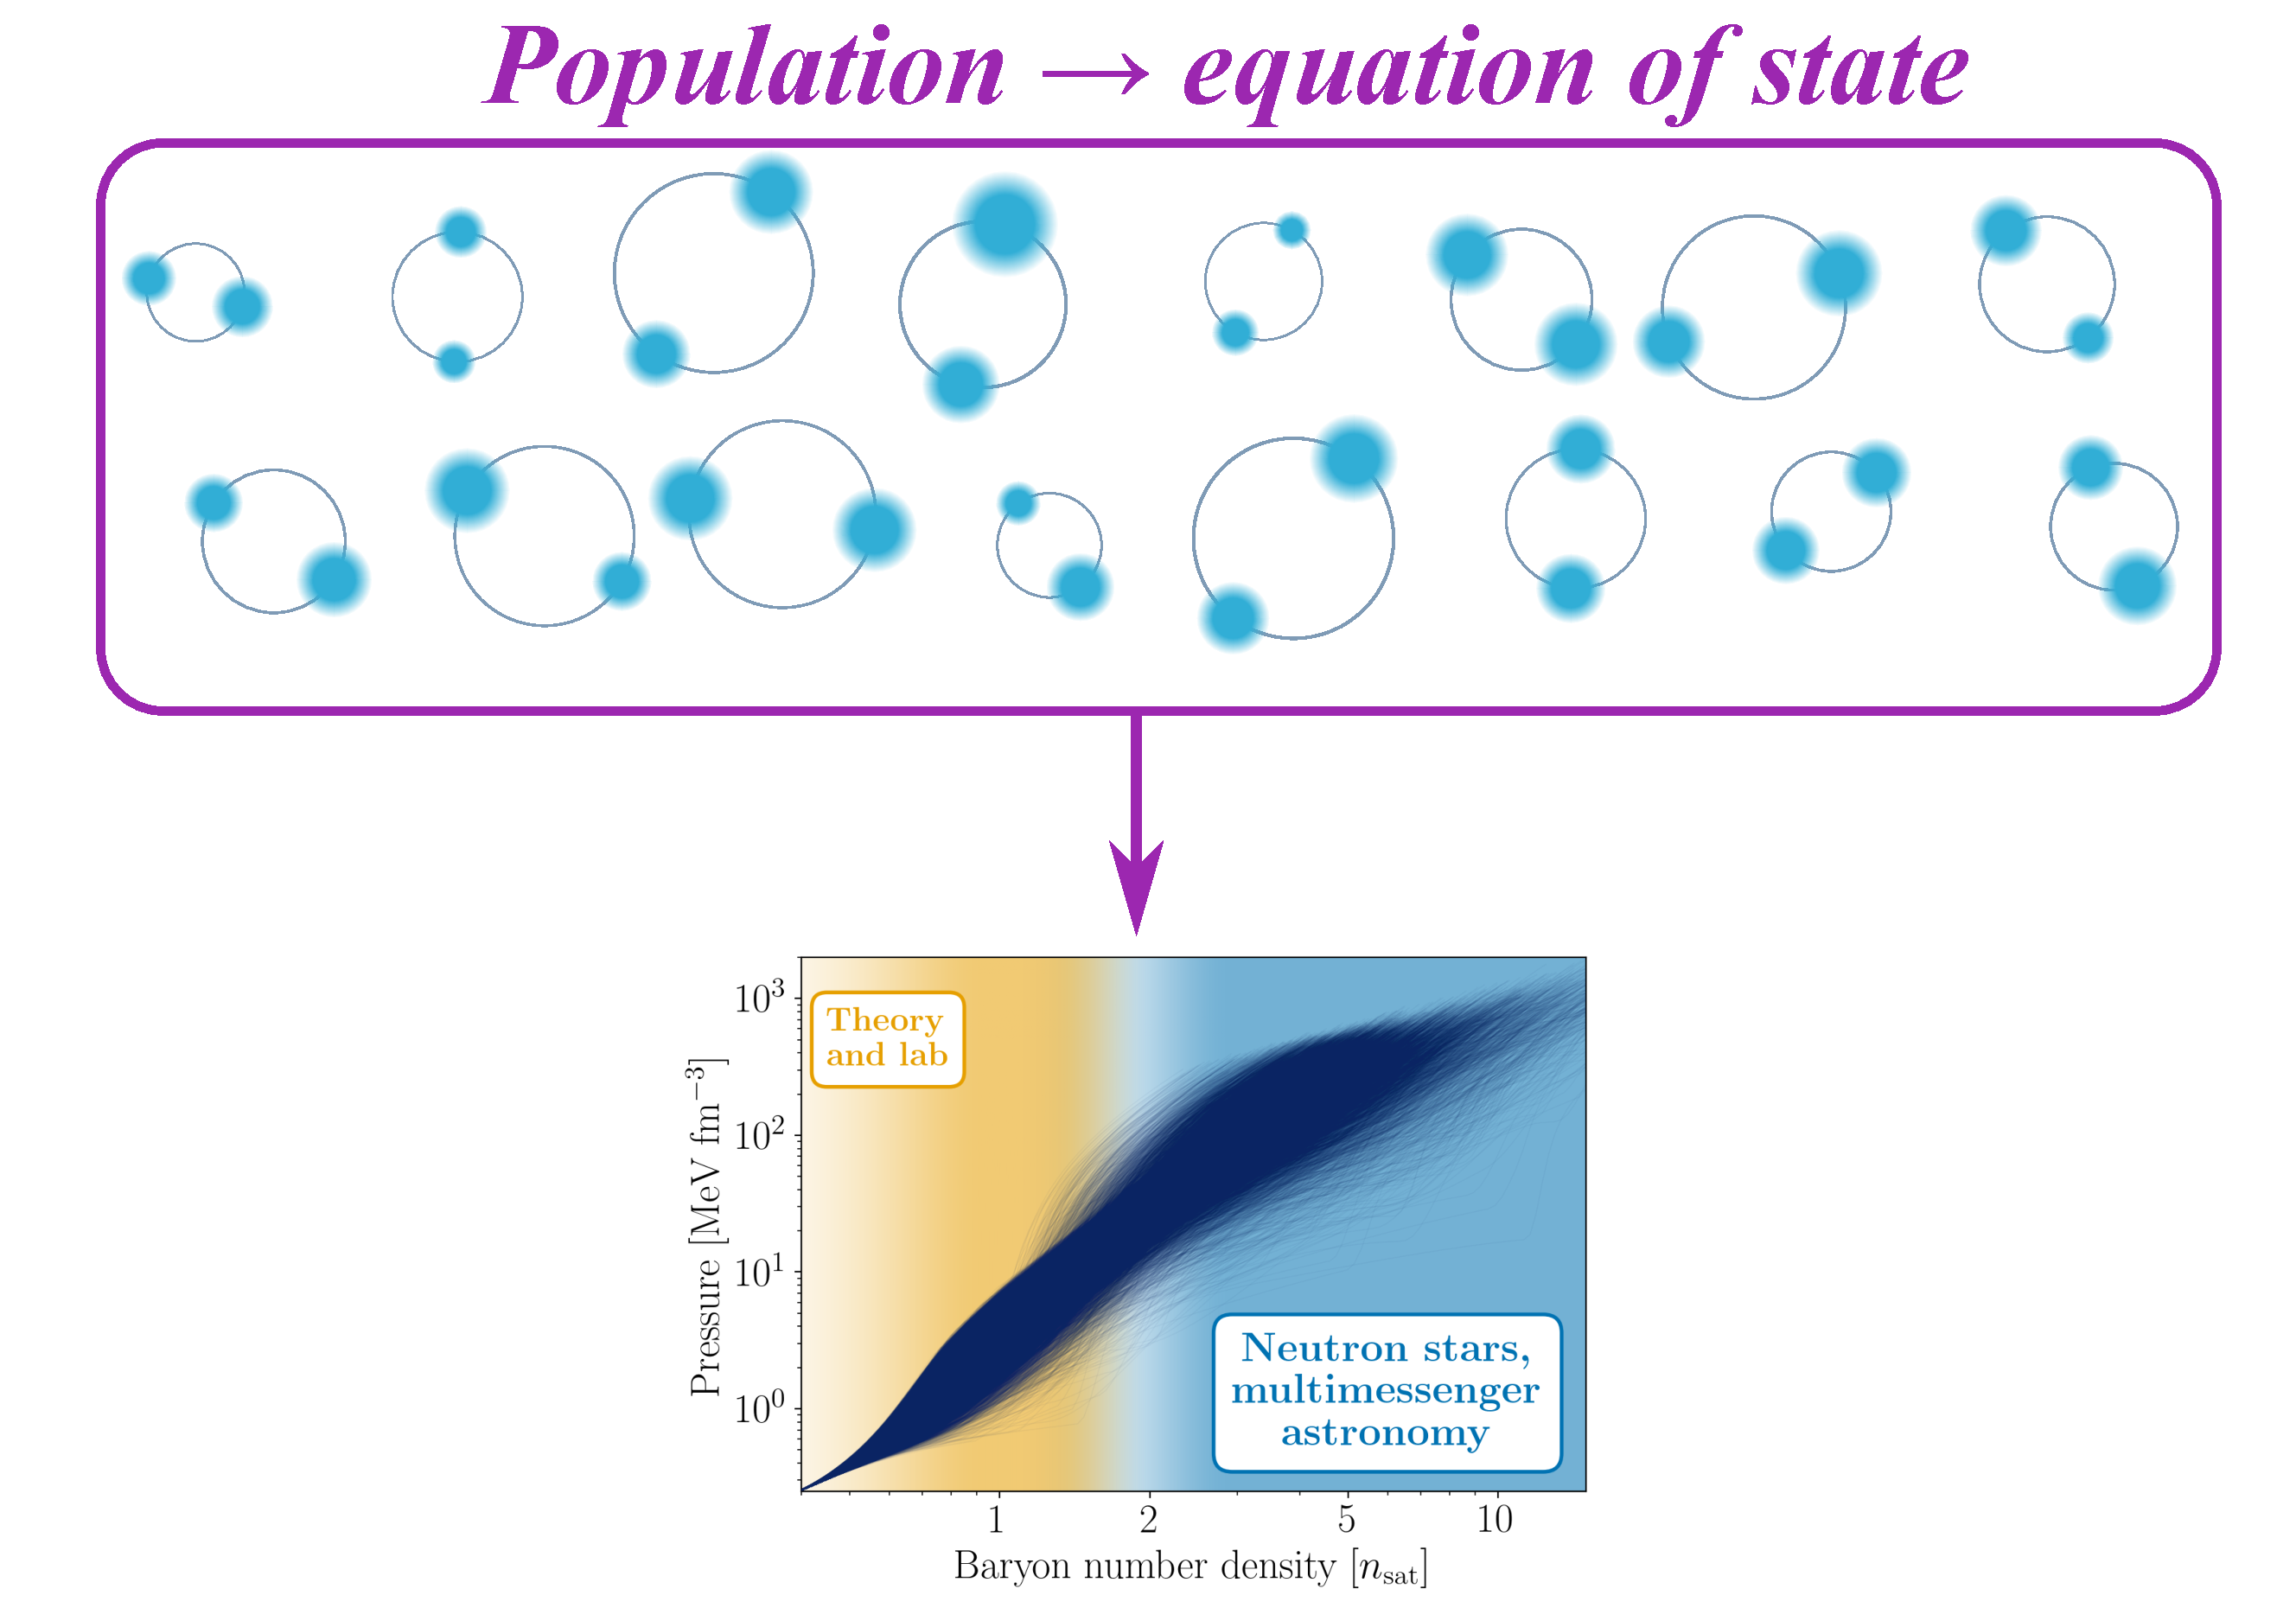
\includegraphics[width=0.9\textwidth]{Inkscape/population_eos.pdf}
  \end{figure}
\end{frame}


\begin{frame}{Equation of state inference with \textsc{jester}}
  \def\x{4mm}
  \def\y{3mm}

  \begin{itemize}
    \item Target: Equation of state (EOS) posterior from $N$ events $d_i$

    \vspace{-2mm}

    \begin{equation*}
      \mathcal{P}(\theta_{\rm{EOS}} | \{d_1, \dots, d_N\}) \propto \mathcal{L}(\{d_1, \dots, d_N\} | \theta_{\rm{EOS}}) \times \pi(\theta_{\rm{EOS}})
    \end{equation*}

    \vspace{2mm}

    \item \textbf{\smcpurple{Sequential Monte Carlo}}: particles from prior to posterior through a sequence of intermediate densities $p_t$

    \vspace{\y}

    \item \textsc{jester} \href{https://github.com/nuclear-multimessenger-astronomy/jester}{\textcolor{black}{\faGithub}}~\cite{Wouters:2025zju}: used by LVK and ET
  \end{itemize}

  \vfill

  \begin{figure}
    \centering
    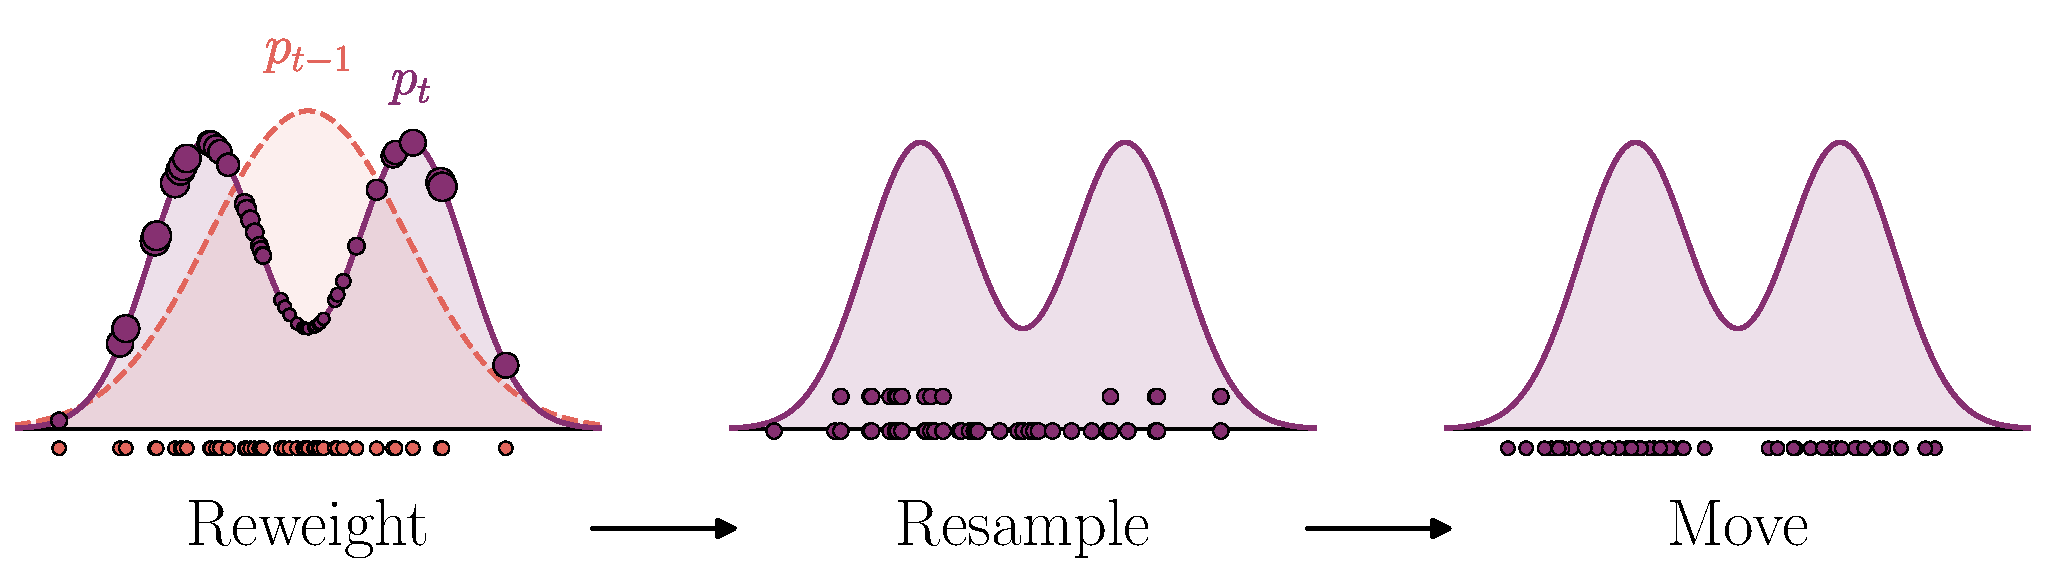
\includegraphics[width=\textwidth]{Figures/smc_steps.pdf}
  \end{figure}

  \vfill

\end{frame}


\begin{frame}{Likelihood tempering vs.\ data tempering}
  \def\x{5mm}
  \def\y{2mm}
  \def\m{-2mm}

  \begin{enumerate}
    \item Likelihood tempering:

    \vspace{\m}
    
    \begin{equation*}
      p_{\red{t}}(\theta) \propto \mathcal{L}(\{d_1, \dots, d_N\} | \theta)^{\red{\beta_t}} \pi(\theta) \, \quad \beta_t: 0 \rightarrow 1
    \end{equation*}

    \vspace{\y}
    
    \item Data tempering:

    \vspace{\m}
    
    \begin{equation*}
      p_{\red{t}}(\theta) \propto \mathcal{L}(\{d_1, \dots, d_{\red{t}}\} | \theta) \pi(\theta) \, \quad t: 1 \rightarrow N
    \end{equation*}
  \end{enumerate}

  \vspace{3mm}

  \begin{figure}
    \centering
    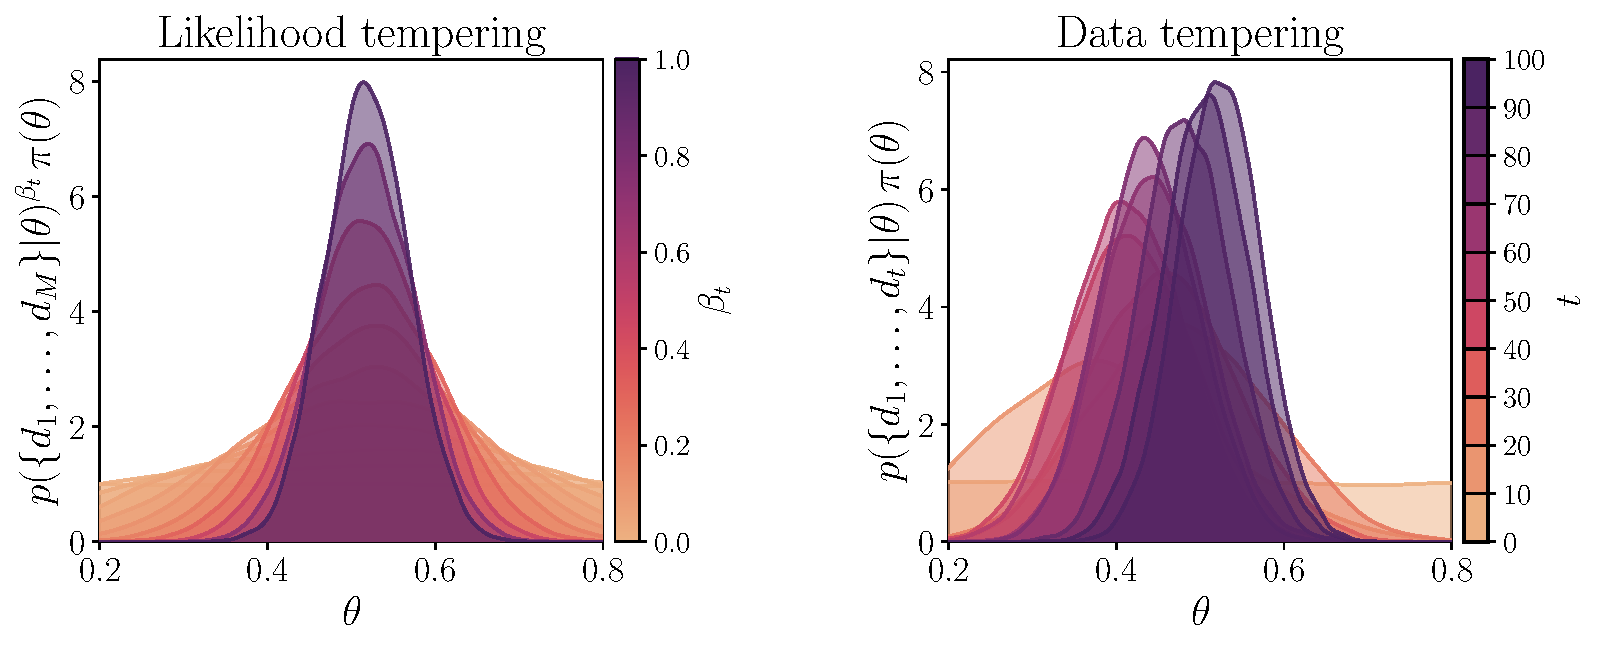
\includegraphics[width=0.95\textwidth]{Figures/smc_temperings.pdf}
  \end{figure}

\end{frame}


\begin{frame}{Adaptive hybrid algorithm (\texttt{2610.07975})}
  \def\x{2mm}

  \begin{itemize}
    \item ET catalogs will grow rapidly: sequentially update posteriors~\cite{wouters2026scalablesequentialinferenceneutron}

    \vspace{\x}

    \item Effective sample size (ESS): metric for adaptive batching

    \vspace{\x}

    \item Use likelihood tempering for robustness
  \end{itemize}

  \vspace{3mm}

  \begin{figure}
    \centering
    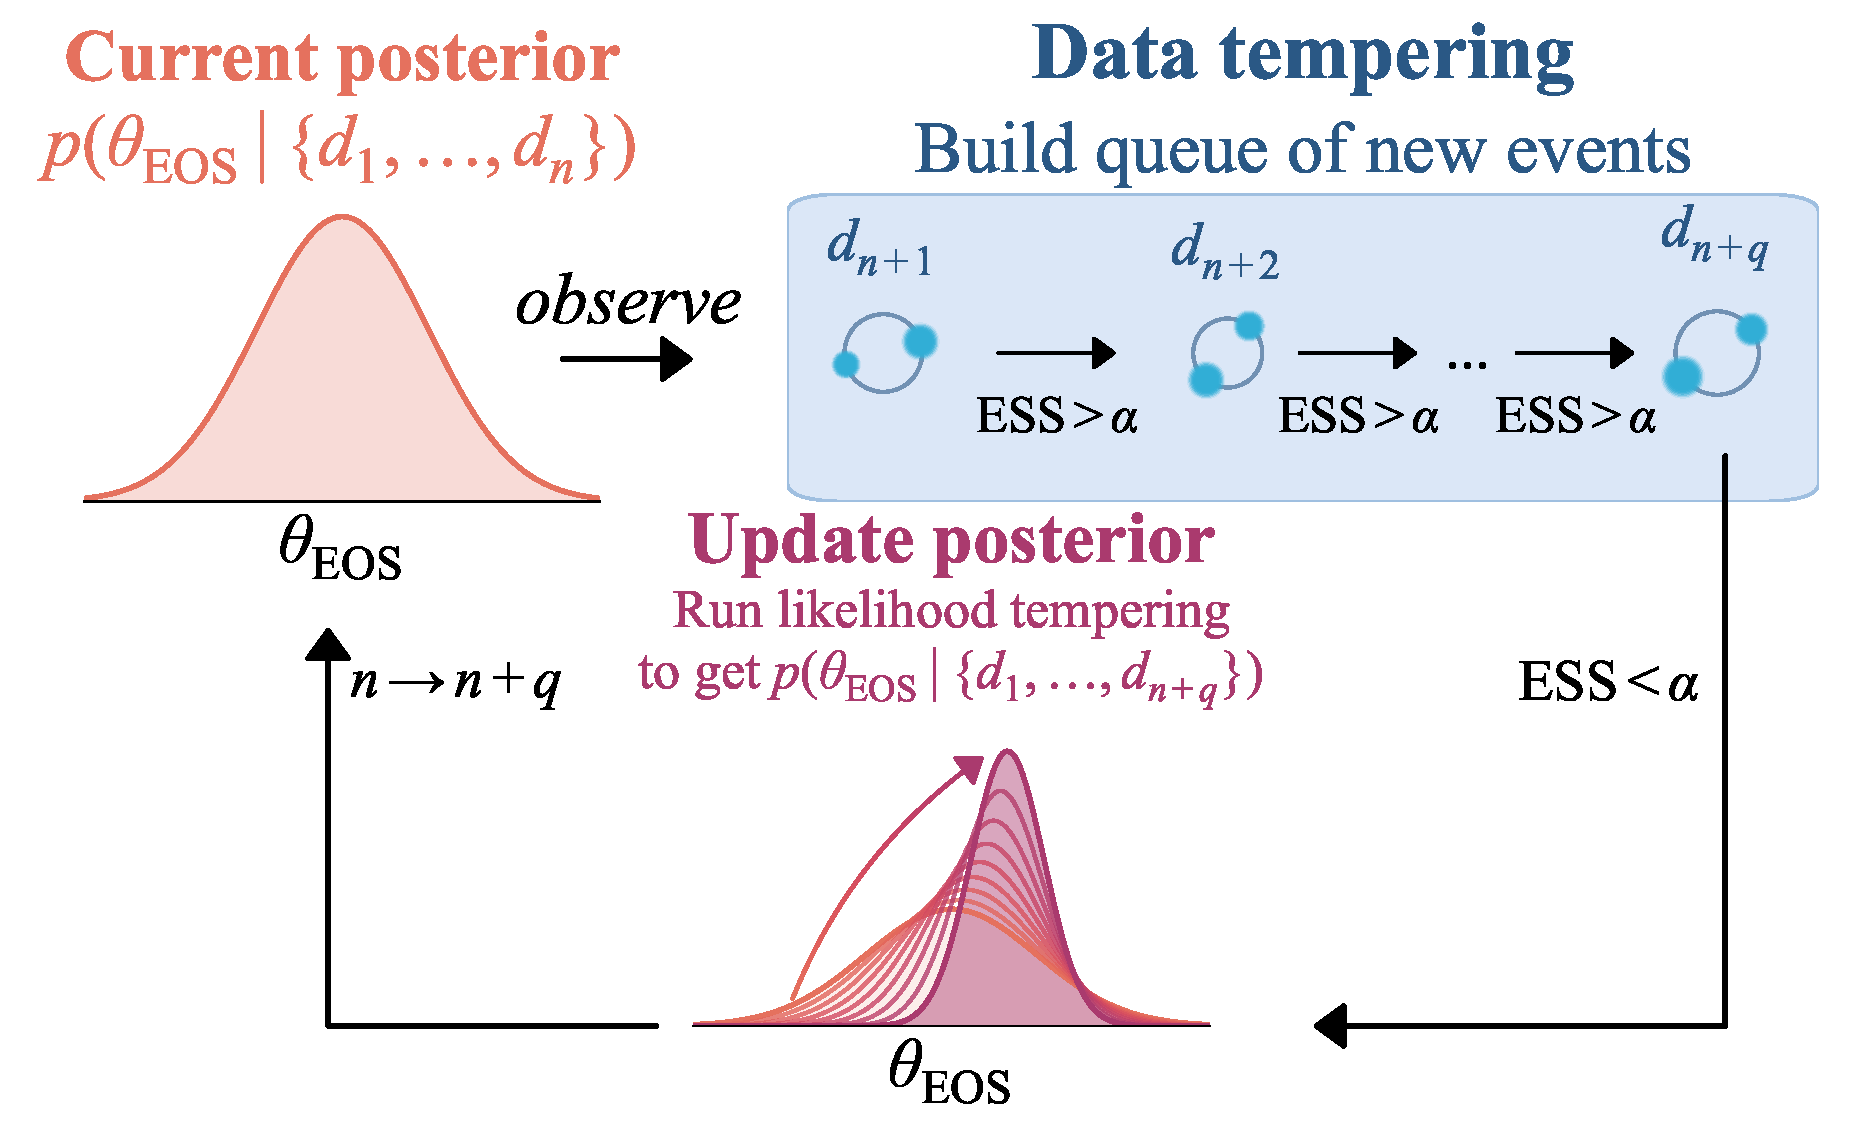
\includegraphics[width=0.775\textwidth]{Figures/fig1_diagram.pdf}
  \end{figure}
\end{frame}

\begin{frame}{Proof of concept (\texttt{2610.07975})}
  \def\x{2mm}
  \def\y{2mm}

  \begin{itemize}
    \item Toy catalogue: $1$ month of binary neutron stars (GW) ($\sim 1500$)

    \vspace{\y}

    \item Runtime $\sim 2$ hrs; expectation for 1 year: $\sim 2$ days

    \vspace{\y}

    \item Processing events `in real time', as we will do it $\sim 10$ years from now!
  \end{itemize}

  \only<1>{
    % \vspace{2mm}
    \begin{figure}
      \centering
      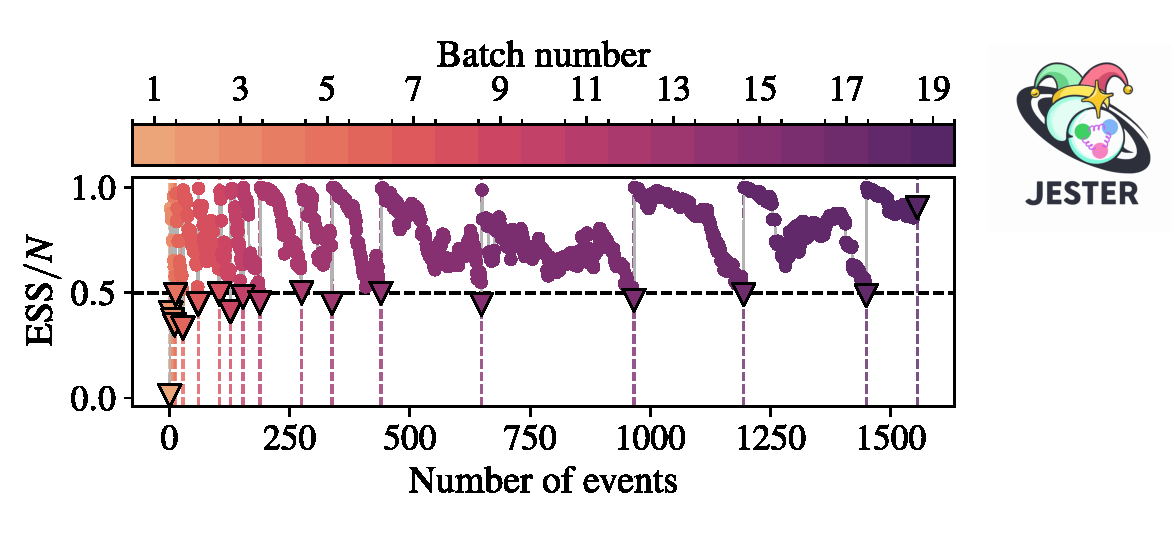
\includegraphics[width=0.90\textwidth]{Inkscape/scalable_jester_smc.pdf}
    \end{figure}
  }
  
  \only<2>{
    % \vspace{2mm}
    \begin{figure}
      \centering
      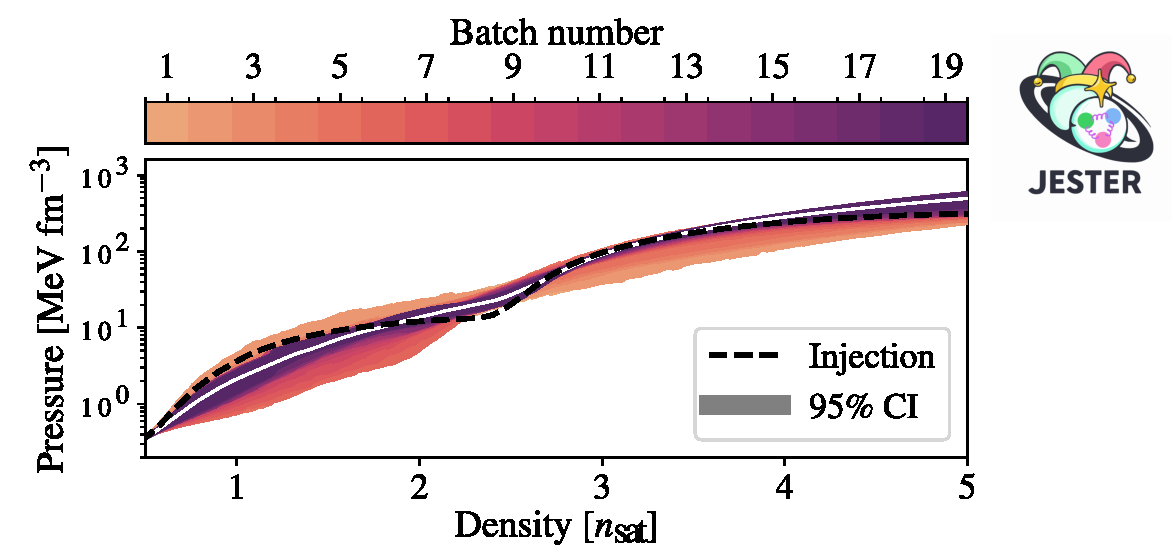
\includegraphics[width=0.875\textwidth]{Inkscape/scalable_jester_eos.pdf}
    \end{figure}
  }
\end{frame}

\begin{frame}[plain, noframenumbering]{}
  \vspace{10mm}
  \begin{figure}
    \centering
    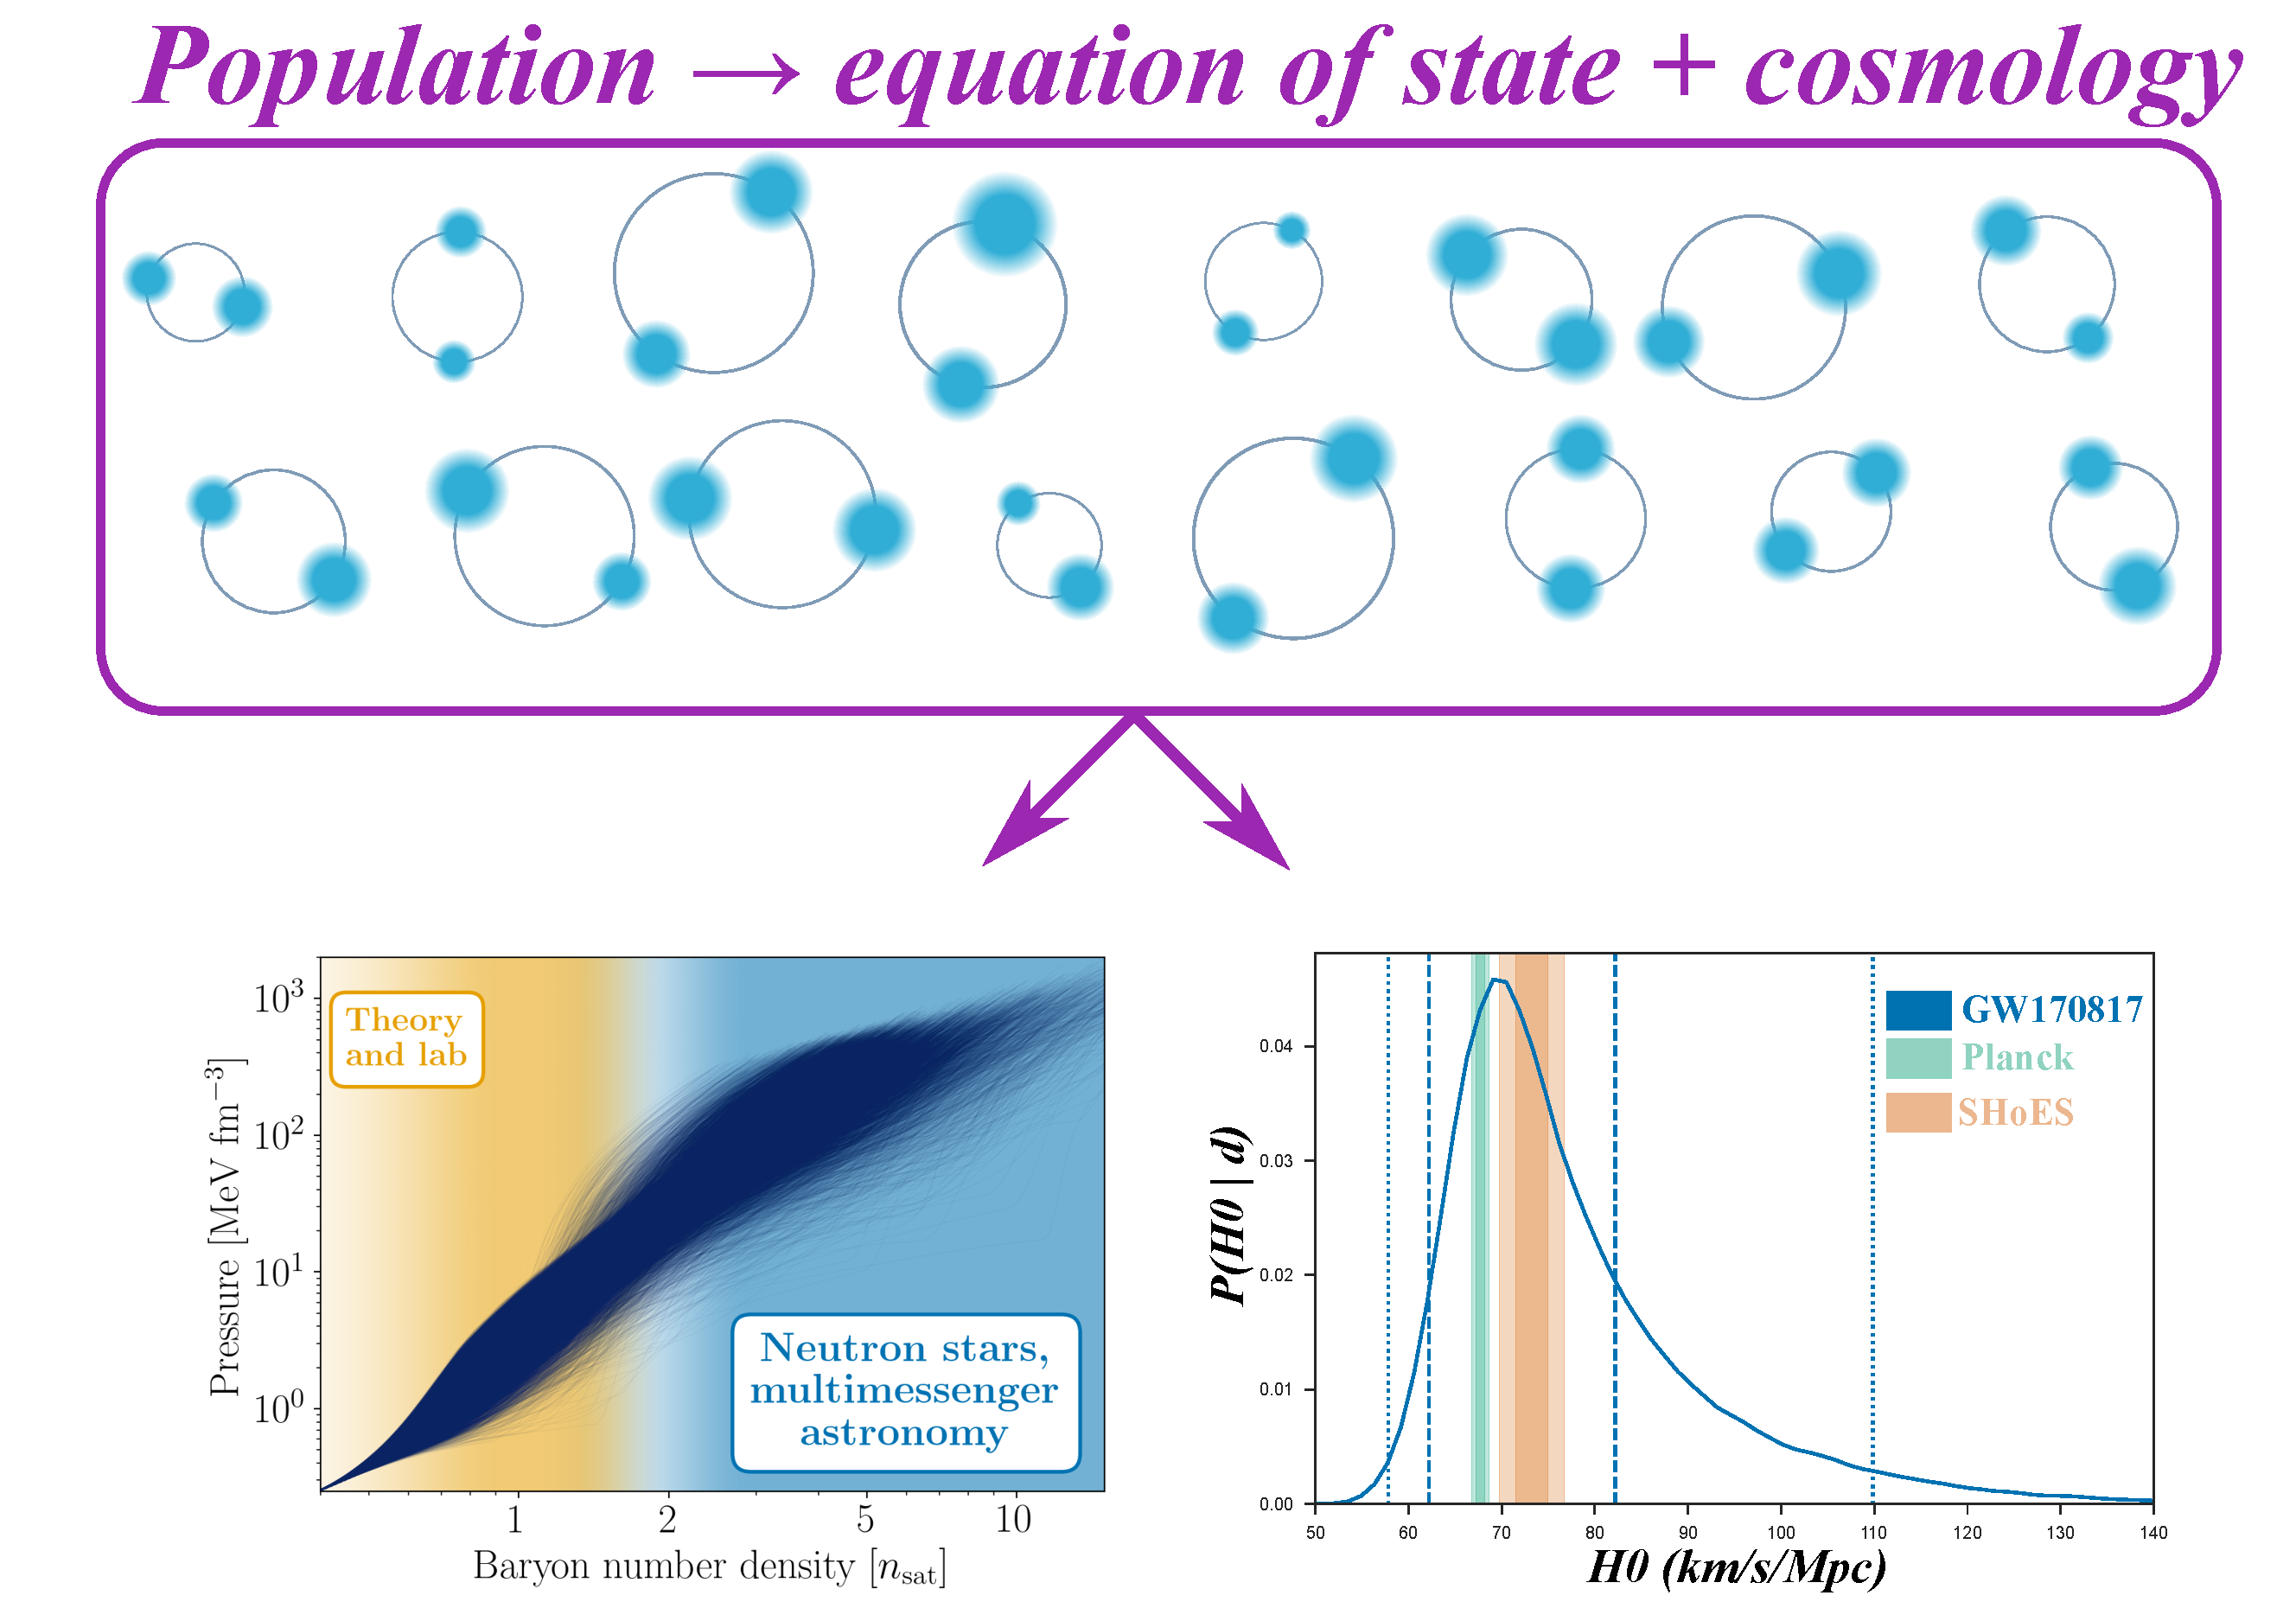
\includegraphics[width=0.9\textwidth]{Inkscape/population_eos_cosm.pdf}
  \end{figure}
\end{frame}

\begin{frame}{Multimessenger forecasts (\texttt{2607.28438})}
  \def\x{2mm}
  \def\y{2mm}

  \begin{itemize}
    \item Multimessenger forecasts ($1$ year of mergers) for population + equation of state + cosmology~\cite{Koehn:2026nin} with \textsc{jester}

    \vspace{\x}
    
    \item GW + kilonova + GRB afterglow on CPU (\textsc{NMMA} \href{https://github.com/nuclear-multimessenger-astronomy/nmma}{\textcolor{black}{\faGithub}})

    \vspace{\x}

    \item Single-event analysis becoming the bottleneck
  \end{itemize}

  \vspace{5mm}

  \begin{figure}
      \centering
      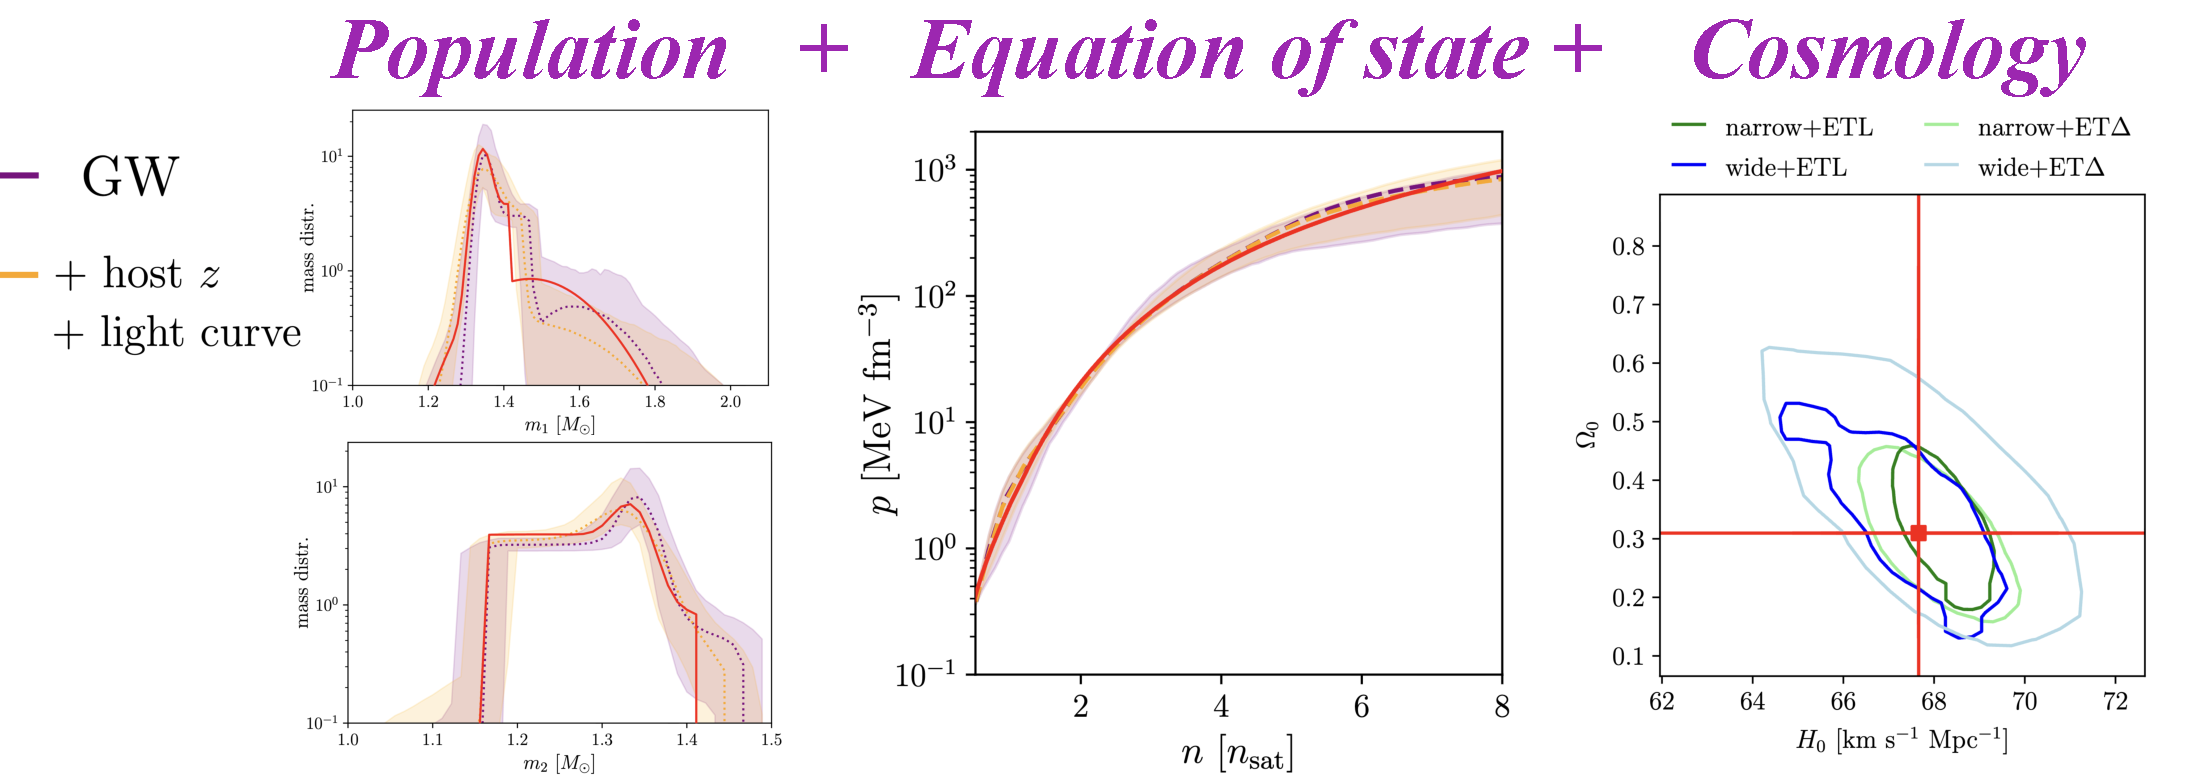
\includegraphics[width=0.95\textwidth]{Inkscape/koehn.pdf}
    \end{figure}
\end{frame}

\begin{frame}{Conclusions}
  \def\x{3mm}
  \def\y{1mm}

  \vspace{-2mm}

  \begin{columns}[T]
  \begin{column}{0.725\textwidth}
  \begin{itemize}
    \item \textbf{Challenge}: ET will see $\mathcal{O}(10^4)$ binary neutron star mergers per year

    \vspace{\x}
    
    \item \textbf{Solution}: GPU $\times$ algorithmic innovations

    \begin{itemize}
      \vspace{\y}
      \item \jaxdarkgreen{\textbf{Single-event}}: slice-within-Gibbs

      \vspace{\y}

      \item \jaxpurple{\textbf{Population}}: sequential Monte Carlo
    \end{itemize}

    \vspace{\x}
    
    \item \textbf{Results}:

    \begin{itemize}
      \vspace{\y}
      \item \jaxdarkgreen{\textbf{\textsc{ripple}, \textsc{jim}}}: 
      \begin{itemize}
        \item LVK signals (and lensing!)
        \item ET under development
      \end{itemize}

      \vspace{\y}

      \item \jaxpurple{\textbf{jester}}
      \begin{itemize}
        \vspace{\y}
        \item Scale to $\mathcal{O}(10^3)$ sources

        \vspace{\y}
        
        \item Multimessenger forecasts
      \end{itemize}
    \end{itemize}
    
    \item Strong BeNL presence!
  \end{itemize}
  \end{column}
  \begin{column}{0.290\textwidth}
    \vspace{-7mm}
    \centering
    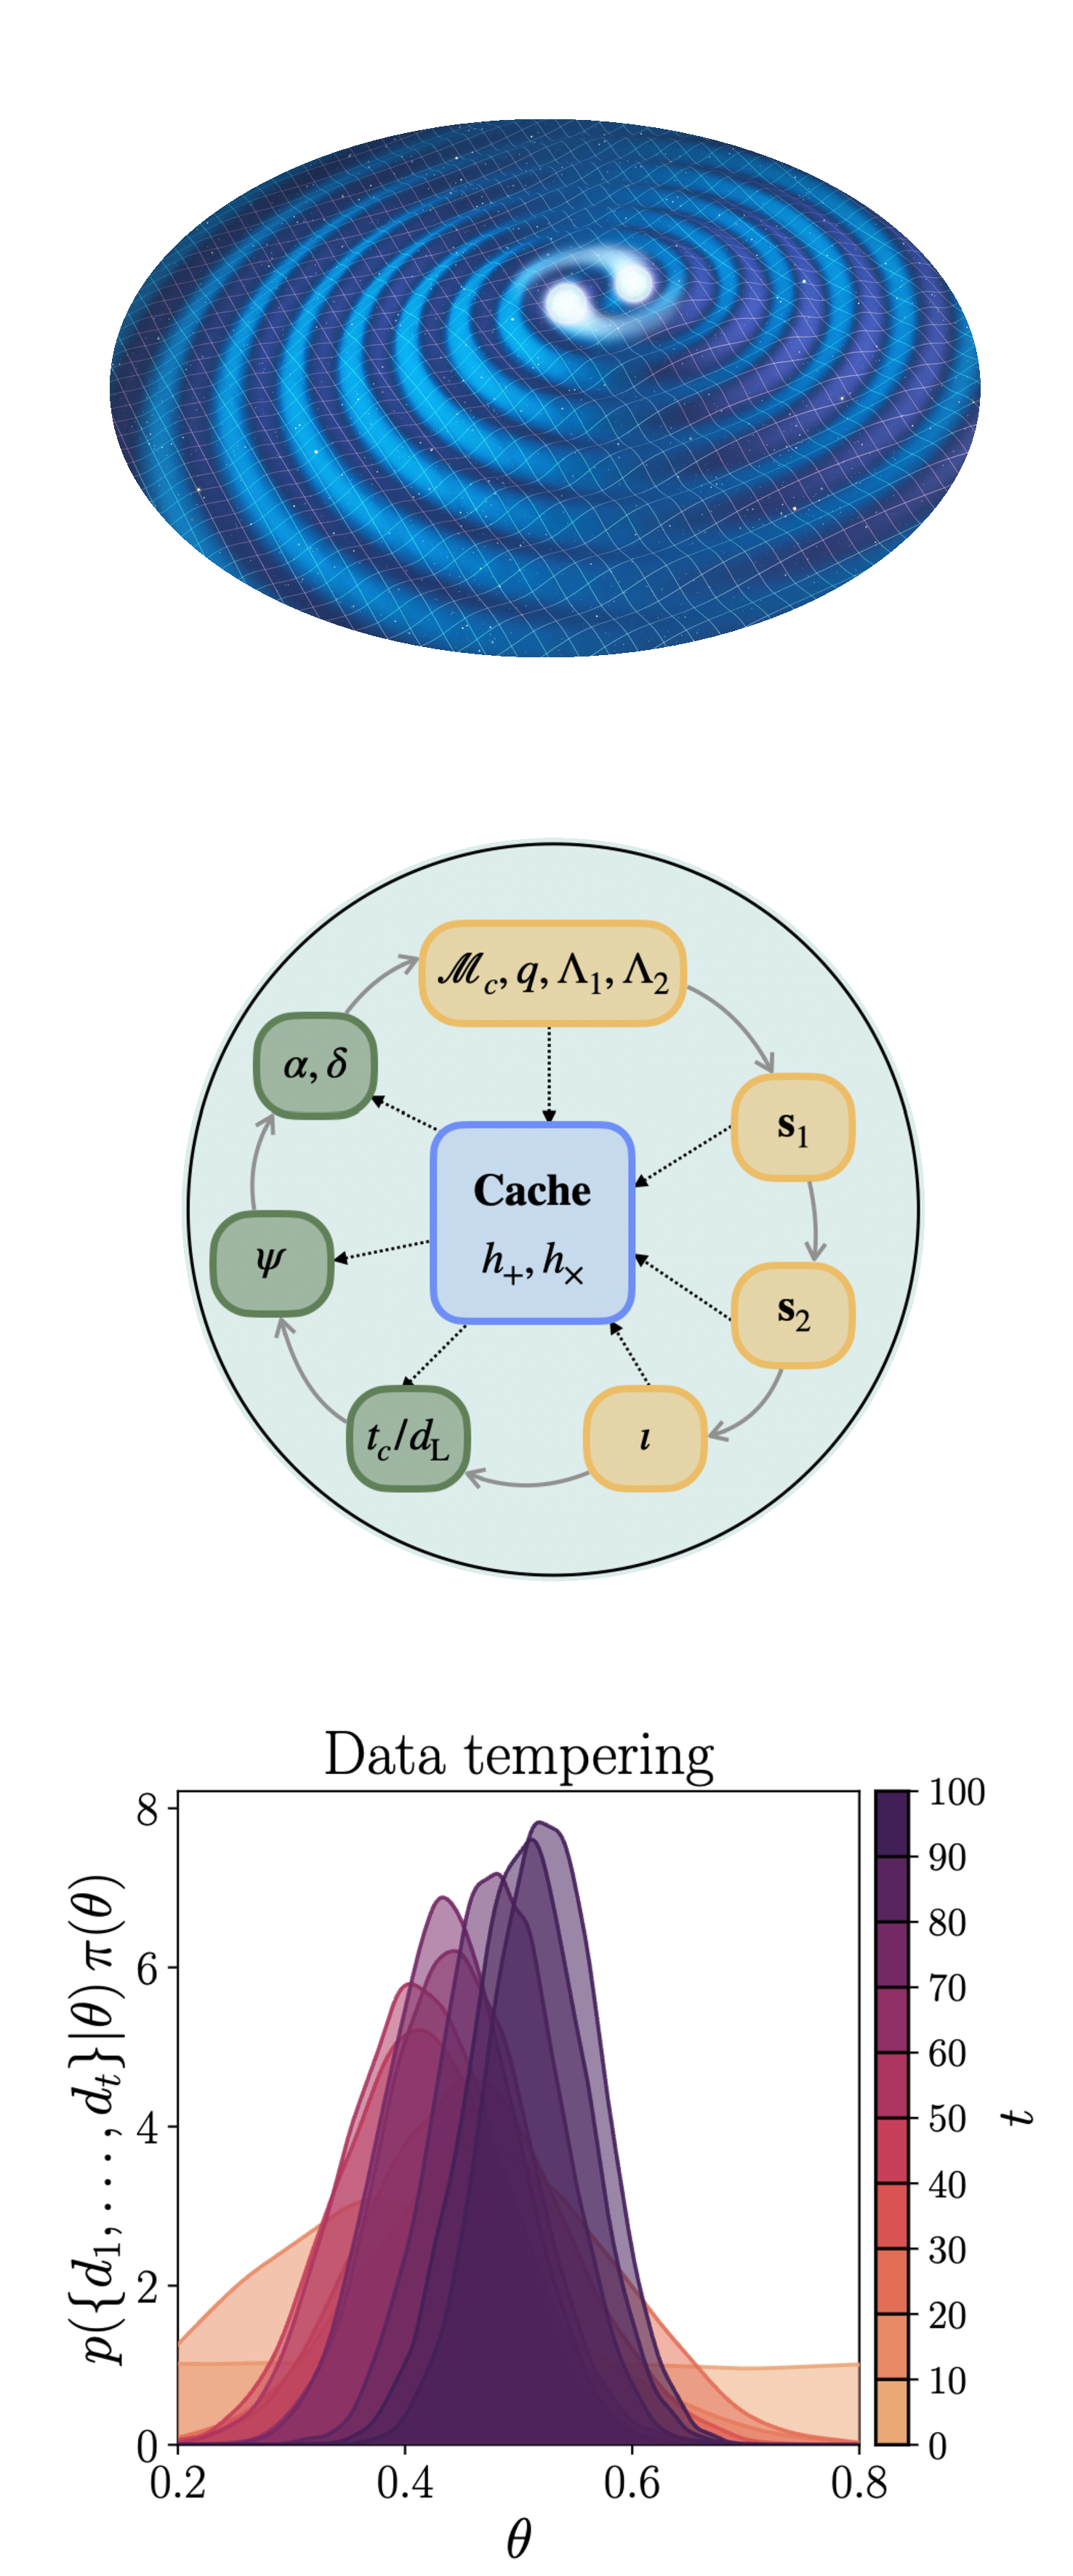
\includegraphics[width=\textwidth]{Inkscape/conclusion.pdf}
  \end{column}
  \end{columns}

\end{frame}

{
\usebackgroundtemplate{\transparent{0.5}{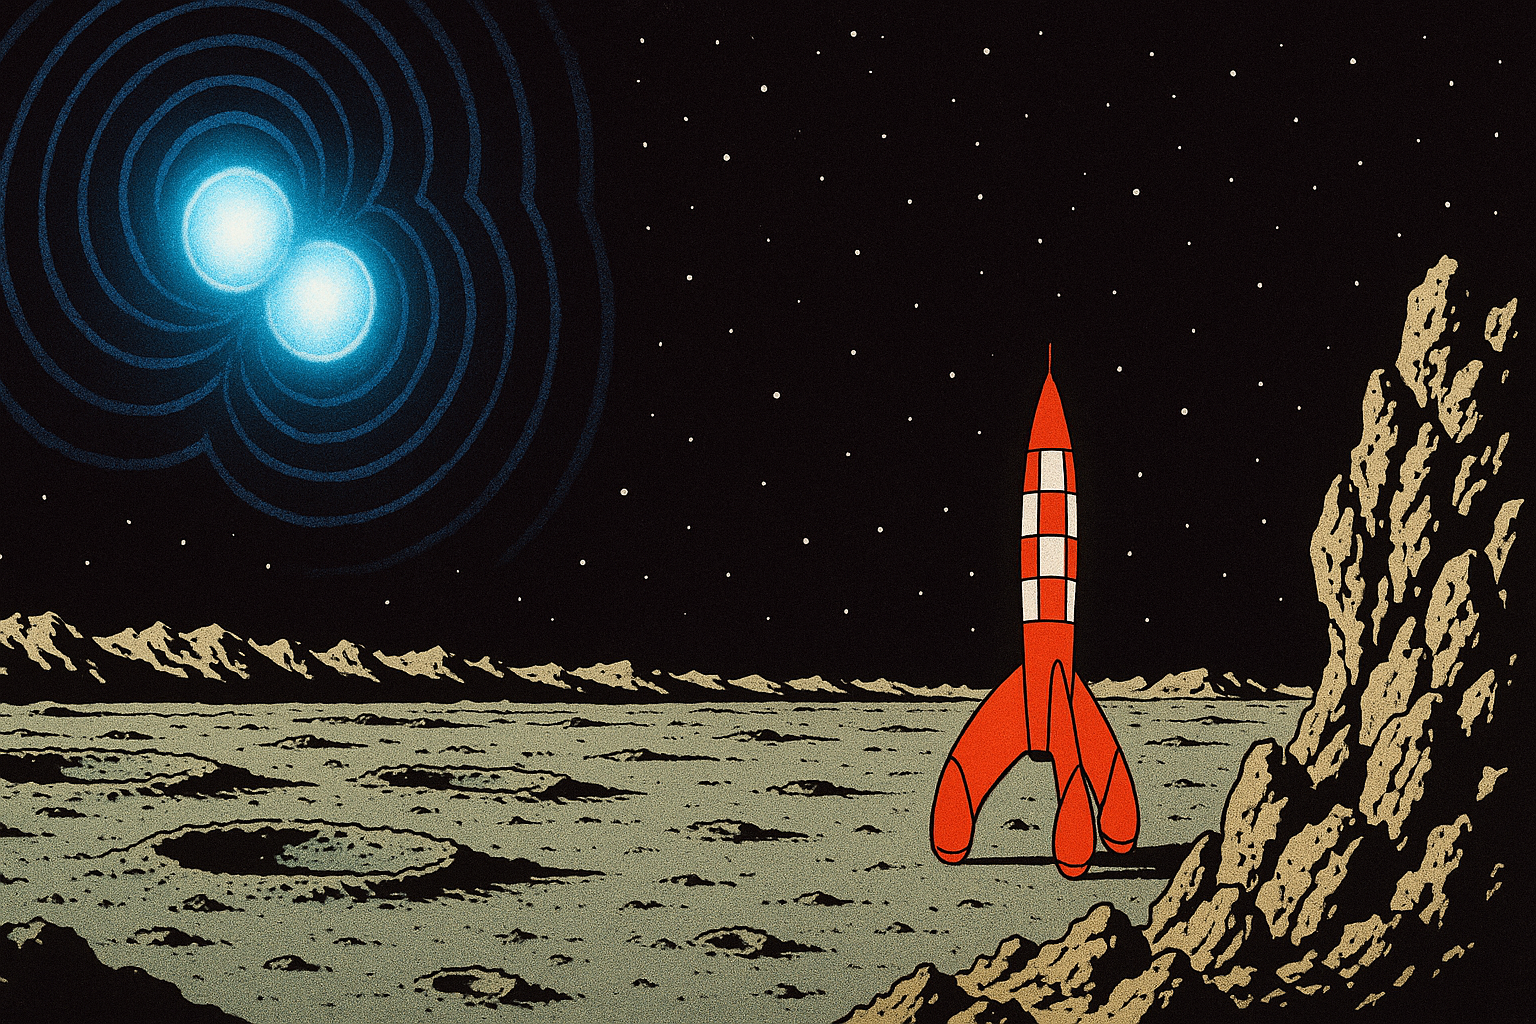
\includegraphics[width=\paperwidth,height=\paperheight]{Figures/tintin_BNS_2.png}}}

\begin{frame}[plain, noframenumbering]

  \begin{tikzpicture}[remember picture,overlay]
    \node[fill=customblue, fill opacity=0.75, text opacity=1, rounded corners=10pt, inner sep=15pt] at ([yshift=2cm]current page.center) {
      \begin{minipage}{0.8\textwidth}
        \centering
        \textbf{Thanks for listening!}
      \end{minipage}
    };
  \end{tikzpicture}

  \end{frame}
}

\begin{frame}{References}

% \nocite{*}
\printbibliography
    
\end{frame}

% ======== APPENDIX  ==========

\appendix

\begin{frame}[plain, noframenumbering]
\vfill
\centering
\textbf{APPENDIX}
\vfill
\end{frame}

\begin{frame}{$\Lambda$ recovery}
  \begin{figure}
    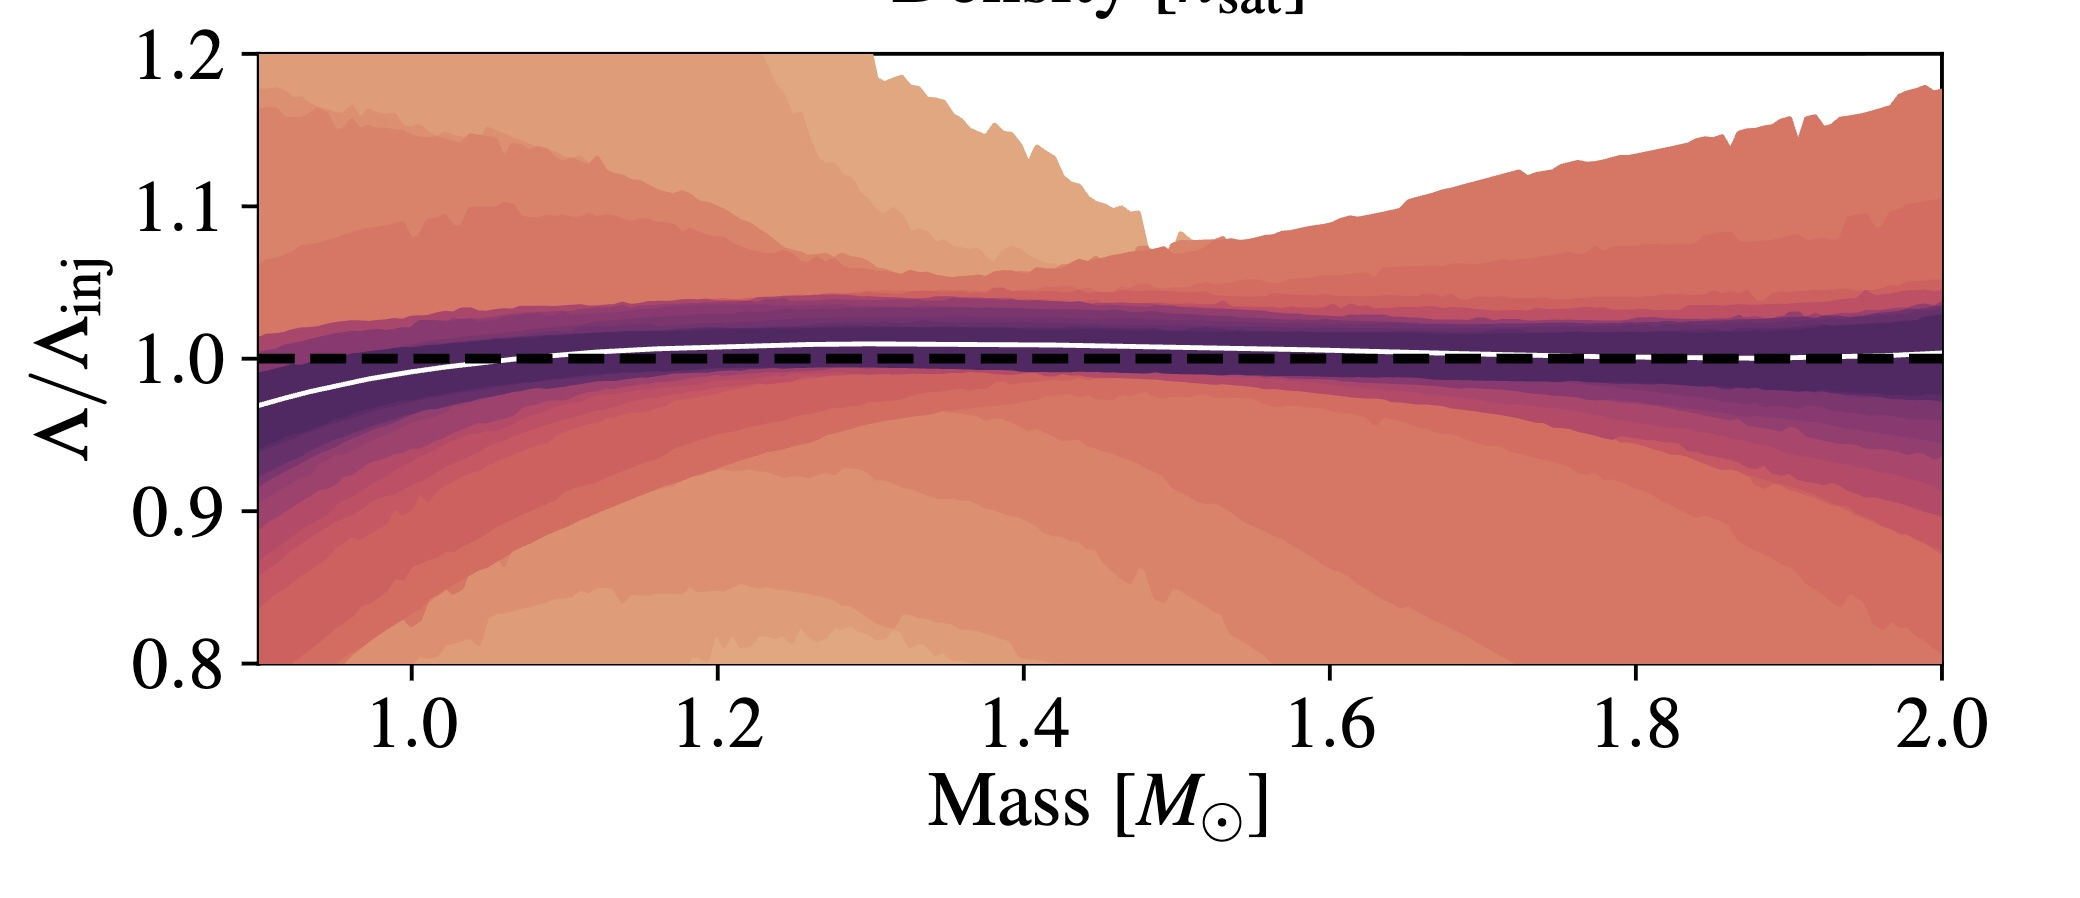
\includegraphics[width=\textwidth]{Figures/lambda_noise.jpg}
  \end{figure}
\end{frame}

\begin{frame}{Zero noise results}
  \begin{figure}
    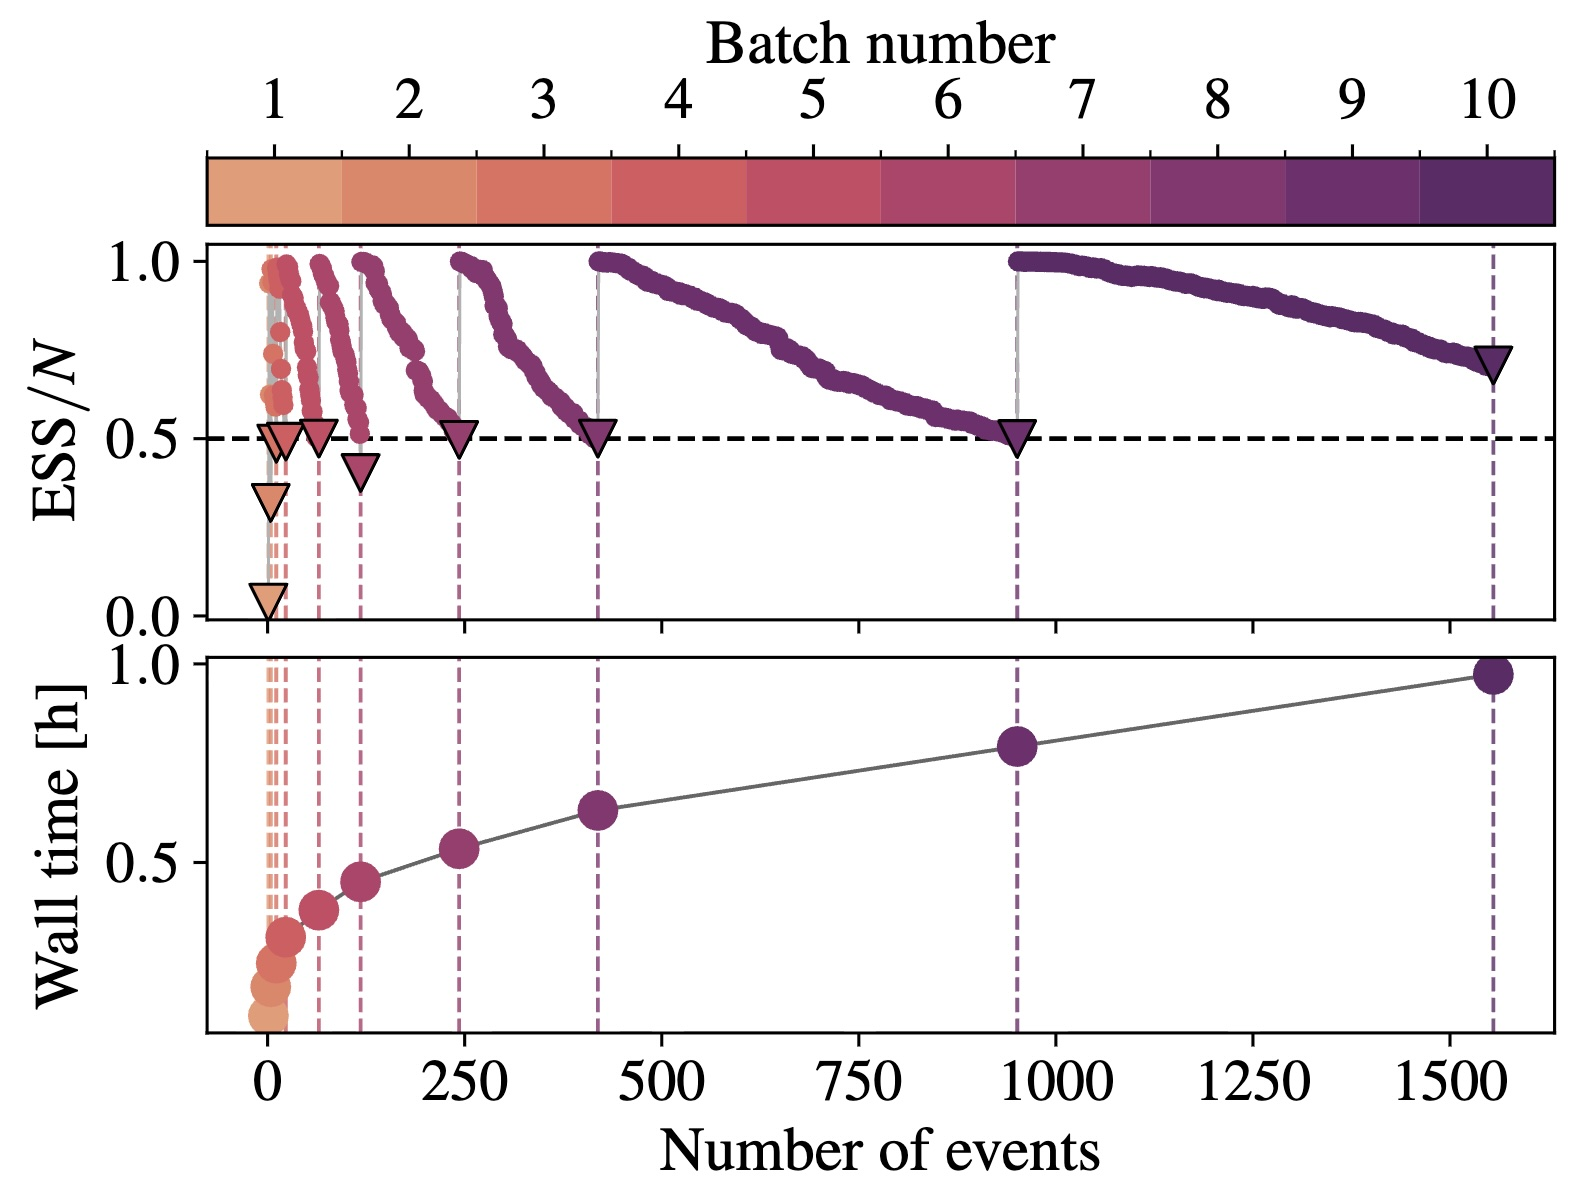
\includegraphics[width=0.75\textwidth]{Figures/no_noise_smc.jpg}
  \end{figure}
\end{frame}

\begin{frame}{Zero noise results}
  \begin{figure}
    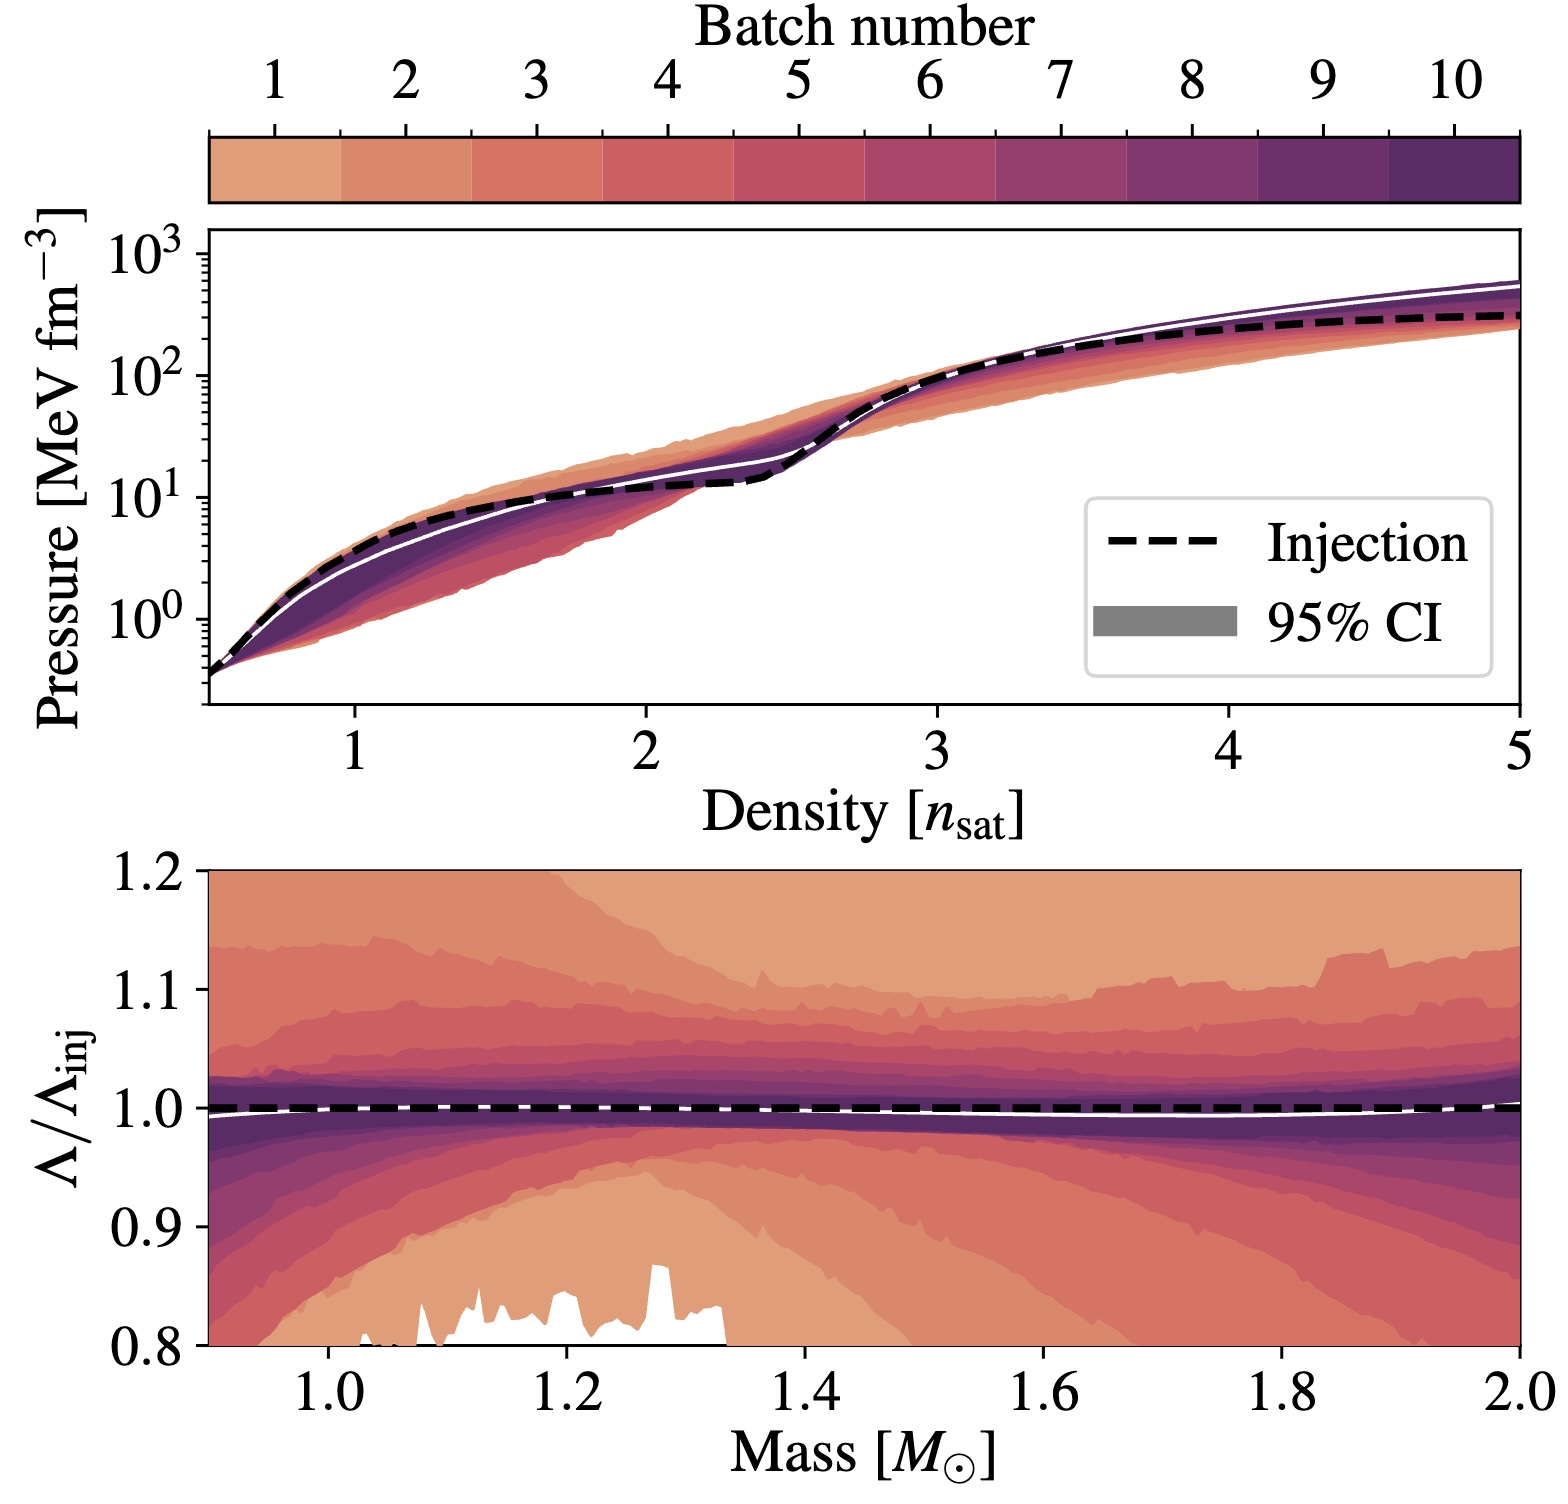
\includegraphics[width=0.65\textwidth]{Figures/no_noise.jpg}
  \end{figure}
\end{frame}
\end{document}